    % ------------------------------------------------------------------------
%
% -------------------      Plantilla_UIS.tex       -----------------------
%
% ------------------------------------------------------------------------
% ------------------------------------------------------------------------
% ------------------------------------------------------------------------
% Versión de plantilla para realización de informes de trabajo de grado
% construida para uso de la Universidad Industrial de Santander.
%
% Reservados todos los derechos
%\\

% Bucaramanga, Colombia
%
% Septiembre 17 de 2018
%
% ------------------------------------------------------------------------
% ------------------------------------------------------------------------
% ------------------------------------------------------------------------
%
% ------------------------------------------------------------------------
\documentclass[letter,oneside,12pt]{report}          % Encabezados 12pt
% ------------------------------------------------------------------------
\usepackage{A-uislatexstyleICONTEC}              % Libreria UIS ICONTEC
\usepackage{citations}
\usepackage{csquotes}
% ------------------------------------------------------------------------
% Ingrese en este punto las librerías específicas de usuario
% ------------------------------------------------------------------------
\usepackage{epsfig}
\usepackage{amsmath}
\usepackage{pdfpages}
\usepackage{amssymb}
\usepackage{subfigure}
\usepackage{graphicx} 
\usepackage[font=small,labelfont=bf,justification=justified]{caption}
\interfootnotelinepenalty=10000
\usepackage{booktabs}
\usepackage[table,xcdraw]{xcolor}
\usepackage{multirow}
\usepackage{bm}


\newcommand\xrowht[2][0]{\addstackgap[.5\dimexpr#2\relax]{\vphantom{#1}}}
\usepackage{pdfpages}
\usepackage{blindtext}
\captionsetup[figure]{name=Figura}
\captionsetup[table]{name=Tabla}


%\bibliographystyle{unsrt}
%\bibliography{xbib}
% ------------------------------------------------------------------------
% Archivo de bibliografía
% ------------------------------------------------------------------------
\bibliography{xbib}
\AtBeginBibliography{\renewcommand*{\mkbibnamefamily}[1]{\MakeUppercase{#1}}}
% ------------------------------------------------------------------------
\begin{document}                                     % Inicio de documento
% ------------------------------------------------------------------------
% Definición silábica de palabras

\graphicspath{ {figures/} }
% ------------------------------------------------------------------------
\hyphenation{}
% ------------------------------------------------------------------------
% Elementos previos al contenido del trabajo
% ------------------------------------------------------------------------
% ------------------------------------------------------------------------
%                                 Portada
% ------------------------------------------------------------------------

\thispagestyle{empty}

\begin{center}

LOCALIZACIÓN DE LESIONES RELACIONADAS CON EL CÁNCER DE PRÓSTATA SOBRE SECUENCIAS MULTIMODALES BP-MRI

\vspace{5cm}

CAMILO EDUARDO GONZÁLEZ GUERRERO\\
\vspace{5cm}

UNIVERSIDAD INDUSTRIAL DE SANTANDER\\
FACULTAD DE INGENIERÍAS FISICOMECÁNICAS\\
ESCUELA DE INGENIERÍA DE SISTEMAS E INFORMÁTICA\\
PROGRAMA DE PREGRADO EN INGENIERÍA DE SISTEMAS E INFORMÁTICA\\
BUCARAMANGA\\
2023\\
\end{center}\vspace{1cm}

\begin{center}

\includegraphics[width=0.9\textwidth]{imgs/logos.png}
\end{center}
%\vspace*{1.5cm}
% \pagenumbering{gobble}

% ------------------------------------------------------------------------
%                              Contraportada
% ------------------------------------------------------------------------

\newpage
\thispagestyle{empty}

\begin{center}

LOCALIZACIÓN DE LESIONES RELACIONADAS CON EL CÁNCER DE PRÓSTATA SOBRE SECUENCIAS MULTIMODALES BP-MRI\vspace{2cm}

CAMILO EDUARDO GONZÁLEZ GUERRERO\\
\vspace{1.5cm}

Trabajo de investigación presentado en cumplimiento de los requisitos para el grado de:\\
Ingeniero de Sistemas e Informática\\\vspace{1.5cm}

Director:\\
Fabio Martínez Carrillo, Ph.D.\\
Doctor en Ingeniería de Sistemas y Computación \vspace{1cm}

Codirector:\\
Juan Andrés Olmos Rojas, M.Sc.\\
Magíster en Matemática Aplicada \vspace{2cm}


UNIVERSIDAD INDUSTRIAL DE SANTANDER\\
FACULTAD DE INGENIERÍAS FISICOMECÁNICAS\\
ESCUELA DE INGENIERÍA DE SISTEMAS E INFORMÁTICA\\
PROGRAMA DE PREGRADO EN INGENIERÍA DE SISTEMAS E INFORMÁTICA\\
BUCARAMANGA\\
2023\\


\end{center}

   % Portada, contraportada, formato de nota y autorización

% ------------------------------------------------------------------------
% ------------------------------------------------------------------------
% ------------------------------------------------------------------------
%                             AGRADECIMIENTOS
% ------------------------------------------------------------------------
% ------------------------------------------------------------------------
% ------------------------------------------------------------------------
\chapter*{AGRADECIMIENTOS}

% Al profesor Fabio Martínez y al profesor Cristian Viáfara por su inmensa dedicación. Sin su apoyo y paciencia no podría haber llevado a término este proyecto. Sus consejos y ajustes emocionales han logrado convertirme en un ingeniero de sistemas más competente, un investigador más capaz y, lo más importante, una mejor persona. \\

% Al grupo de investigación $BIVL^{2}ab$ por abrirme las puertas y brindarme no solo las herramientas necesarias para llevar a cabo esta investigación, sino también un equipo de personas maravillosas que me han orientado y aconsejado a lo largo de este camino. \\

% A la escuela de ingeniería de sistemas y a su equipo de profesores y profesionales que han aportado su valioso grano de arena en mi camino como ingeniero de sistemas.\\

% A la Universidad Industrial de Santander por recibirme durante todo este camino y brindarme la oportunidad de crecer profesional y personalmente.\\




\newpage 
\chapter*{DEDICATORIA}

% \begin{flushright}
% \textit{A Dios, por darme vida para seguir luchando por mis sueños}.\\[0.7cm]

% \textit{A mi madre, por su confianza y amor incondicional. Por ser mi ancla, mi principal soporte y la persona mas importante en mi vida.}.\\[0.7cm]

% \textit{A mi familia por creer en mi, por apoyarnos en todas las circunstancias que han pasado y darnos la mano a mi mamá, a mi hermano y a mi, cuando nadie mas lo hizo.}\\[0.7cm]

% \textit{Al profesor Fabio Martínez y sus ajustes emocionales, a Brayan, Aleja, Edgar, Franklin, Santi, Olmos, Guaya, Lina, Yesid, y todo el team $BIVL^{2}ab$ por su acompañamiento y consejos durante todo el proceso. Hicieron de este viaje un proceso bonito.}\\[0.7cm]

% \textit{A mis amigos de toda una vida Patico, Niño, Gio, Pao, Buenito y Gimena, Dersiton, y Wilmer quienes han hecho todo este camino mas ameno de transitar, quienes siempre han estado ahí para escucharme y ayudarme a crecer como persona. }\\[0.7cm]

% \textit{A todas las personas que han dejado un aporte, positivo o negativo, en mi vida y me han ayudado a ser lo que soy, desde el agradecimiento y el perdón.}\\[0.7cm]

% \textit{A todas las personas que luchan por construir un mejor país.}\\[1cm]

% \textit{\textbf{William David Romero Serrano.}}\\[0.7cm]


% \end{flushright}


\newpage  
% ------------------------------------------------------------------------

\tableofcontents


\addto\captionsenglish{% Replace "english" with the language you use
  \renewcommand{\tableofcontentsname}%
    {Whatever}%
}
% Tabla de contenido

% ------------------------------------------------------------------------

\listoffigures                        % Lista de figuras, tablas y anexos
\listoftables
%\listofanexo
% ------------------------------------------------------------------------
% Contenido del Informe
% ------------------------------------------------------------------------
% ------------------------------------------------------------------------
% ------------------------------------------------------------------------
% ------------------------------------------------------------------------
%                                Abstract
% ------------------------------------------------------------------------
% ------------------------------------------------------------------------
% ------------------------------------------------------------------------
\chapter*{ABSTRACT}

\footnotesize{
\begin{description}
  \item[TITLE:] Localization of prostate cancer-related lesions on multimodal bp-MRI sequences. \astfootnote{Research work}
  \item[AUTHOR:] Camilo Eduardo González Guerrero \asttfootnote{Faculty of Physics-Mechanics Engineering. School of Systems Engineering and Informatics. Advisor: Fabio Martínez, Ph.D. Co-advisor: Juan Andrés Olmos Rojas, M.Sc.}
  \item[KEYWORDS:] Prostate cancer, bpMRI, csPCa lesion, multimodal
  
  \item[DESCRIPTION:] 
Prostate cancer is the second cancer with the highest incidence in men worldwide. In Colombia, for example, the death rate is around 11.6 cases per 100,000 inhabitants. Nowadays, the study of prostate lesions through biparametric magnetic resonance imaging is a standard criterion for the detection and diagnosis of prostate cancer, even in early stages. However, the localization of these lesions remains subjective and their characterization reports low levels of sensitivity. This is why computational mechanisms are nowadays key for the localization, diagnosis and triage of prostate cancer on bp-MRI studies. In this proposal we intend to develop a deep learning tool to localize prostate lesions from the assessment of multiple MRI parameters. For the above, a dataset properly annotated by experts will be selected, a deep learning tool will be adjusted and adapted. The proposed schema is expected to be validated in terms of its ability to localize lesions and discriminate them according to the stratification of the dataset.   

 


\end{description}
}\normalsize                                               % Resumen
% ------------------------------------------------------------------------
% ------------------------------------------------------------------------
% ------------------------------------------------------------------------
%                                Resumen
% ------------------------------------------------------------------------
% ------------------------------------------------------------------------
% ------------------------------------------------------------------------

\chapter*{RESUMEN}

\footnotesize{
\begin{description}
  \item[TÍTULO:] Localización de lesiones relacionadas con el cáncer de próstata sobre secuencias multimodales bp-MRI\astfootnote{Trabajo de investigación}
  \item[AUTOR:] Camilo Eduardo González Guerrero\asttfootnote{Facultad de Ingenierías Fisicomecánicas Escuela de Ingeniería de Sistemas e Informática. Director: Fabio Martínez Carrillo, Ph.D. Codirector: Juan Andrés Olmos Rojas, M.Sc. }
  \item[PALABRAS CLAVE:] Cáncer de próstata, localización, lesión csPCa, bpMRI, multimodal.
  \item[DESCRIPCIÓN:] 
El cáncer de próstata es el segundo cáncer con mayor incidencia en hombres a nivel mundial. En Colombia, por ejemplo, la tasa de defunción es de alrededor de 11.6 casos por cada 100 mil habitantes. Hoy en día, el estudio de lesiones prostáticas mediante resonancia magnética biparamétrica es un criterio estándar para la detección y diagnóstico del cáncer de próstata, incluso en estadios tempranos. Sin embargo, la localización de estas lesiones sigue siendo subjetiva y su caracterización reporta bajos niveles de sensibilidad. Es por ello por lo que los mecanismos computacionales son hoy en día claves para la localización, diagnóstico y triage del cáncer de próstata sobre los estudios bp-MRI. En esta propuesta se pretende desarrollar una herramienta de aprendizaje profundo para localizar lesiones prostáticas a partir de la observación de múltiples parámetros de la resonancia. Para lo anterior, se seleccionará un conjunto de datos debidamente anotado por expertos, se ajustará y adaptará una herramienta de aprendizaje profundo. Se espera validar el esquema propuesto en cuanto a la capacidad de localizar lesiones y discriminarlas según la estratificación del conjunto de datos. 
 
\end{description}
}\normalsize
% ------------------------------------------------------------------------                                               % Abstract
% ------------------------------------------------------------------------
% Capítulos
% ------------------------------------------------------------------------
% ------------------------------------------------------------------------
% ------------------------------------------------------------------------
% ------------------------------------------------------------------------
%                              Introducción
% ------------------------------------------------------------------------
% ------------------------------------------------------------------------
% ------------------------------------------------------------------------


\nnchapter{INTRODUCCIÓN} %max 5 pags
% ------------------------------------------------------------------------
% ------------------------------------------------------------------------


% 1er parrafo. Impacto 

El cáncer de próstata (PCa) es el segundo cáncer más común en hombres y en la mayoría de los países se establece como el más diagnosticado. En 2020, a nivel global hubo 1.4 millones de casos nuevos y más de 300.000 fallecimientos. Además, se estima que las muertes asociadas a este cáncer se duplicarán para el año 2040 \myfootcite{Sung2021}. A nivel mundial, el 6.8\% de las muertes por cáncer en hombres son por cáncer de próstata, mientras que en Colombia esta cifra ha presentado un incremento constante en los últimos 20 años, siendo actualmente la causante del 14.5\% de las muertes asociadas a cáncer en hombres  \myfootcite{Sung2021,asivamosensalud}.\par

% -- 2do parrafo. Problema y situacion actual (Como lo hacen y problemas...). 
En la práctica clínica, se busca identificar lesiones clínicamente significativas de cáncer de próstata (csPca, por sus siglas en inglés), cuya detección temprana permite reducir el número de lesiones agresivas y la cantidad de muertes asociadas a este cáncer \myfootcite{uro2020014}. Por ello, un diagnóstico preciso y oportuno es relevante para diseñar mejores tratamientos que impacten positivamente en el paciente. A la fecha, los métodos mas utilizados durante la rutina clínica para el diagnóstico inicial, o sospecha de PCa, son el examen de sangre de antígeno prostático (prostate specific antigen, PSA) y el examen rectal digital (digital rectal exam, DRE) \myfootcite{Ftterer2015,Wang2021,Smith2004}. Sin embargo, se ha mostrado que el examen PSA presenta una baja especificidad, alcanzando cifras cercanas al 20\% \myfootcite{Merriel2022}. Por otra parte, el DRE es un método invasivo, altamente dependiente de la experiencia del experto y no permite examinar zonas importantes de la glándula prostática, ignorando así potenciales lesiones csPCa \myfootcite{david2022prostate,Naji2018}.\par


% ------ BPMRI as potential.  
El análisis de secuencias de resonancia magnética multi-paramétrica (MP-MRI) se ha constituido en los últimos años como una alternativa prometedora para soportar el diagnóstico temprano en una fase previa a la biopsia \myfootcite{Deniffel2021}. Estas secuencias se usan como una herramienta estándar para el diagnóstico o el tamizaje (`screening') poblacional en diferentes regiones en el mundo \myfootcite{10.1001/jamaoncol.2020.7456,Saar2020}. En especial, permiten caracterizar lesiones, incluso en regiones alejadas de la pared rectal y zona transicional \myfootcite{murphy2013expanding,Stabile2019}. Sin embargo, el enfoque MP-MRI implica la utilización de agentes de contraste, que pueden tener efectos secundarios como malestar general o irritación en la piel, debido a la inyección del agente de contraste. Así mismo, requiere un tiempo considerable para generar su secuencia de imágenes, y por si fuera poco, ya se ha relatado sobre una posible no evidencia estadística significativa con el uso de su secuencia (DCE) \myfootcite{Behzadi2018,GraciaBara2022,Schoots2021,Tan2015}. De manera que, el uso de secuencias de resonancia magnética bi-paramétricas (bp-MRI) ha emergido como una alternativa, que,  en comparación con las secuencias MP-MRI, resultan hasta tres veces más rápidas, no requieren agentes de contraste y tienen una precisión equiparable en el soporte al diagnóstico \myfootcite{Pecoraro2021,Obmann2018,Alver2022,Steinkohl2018}.
A pesar de ello, el análisis de lesiones en secuencias MRI es afectado por la variabilidad que existe entre lecturas por parte de diferentes radiólogos, subjetividad que puede inducir errores en la caracterización y localización de lesiones csPCa. Particularmente, la caracterización de estas lesiones en secuencias bp-MRI es una tarea compleja para los radiólogos, su competencia se logra con experiencia, tanto en años, como en número de interpretaciones \myfootcite{Salka2022,Kang2021}. Sin embargo, 
no son muchos los radiólogos que cuentan con esta experiencia, y en eventuales diagnósticos masivos, ya existe preocupación por posible escasez de personal \myfootcite{Mata2021,Rimmer2017}. A propósito de lo anterior, se han propuesto ambiciosos programas para fortalecer tareas de tamizaje basados en estudios MRI que permitan mitigar la mortalidad asociada a este cáncer \myfootcite{Bratt2023}. Ahora bien, en relación a resultados coetáneos, de programas de tamizaje previo, se evidencia que las labores de clasificación, o determinación de un grado en una escala para este tipo de cáncer no han sido muy efectivas, pues no hay evidencia de disminución en la mortalidad \myfootcite{Hamdy2023}. Anejando por lo dicho, para una correcta caracterización, resultarían necesarias herramientas que especialicen la tarea de localización de lesiones sobre estas secuencias MRI.\par

%existen metodos computacionales....de clasificacion... pero estos parten de una localización
En los últimos años, el uso de herramientas computacionales ha surgido como una herramienta prometedora para ayudar en el diagnóstico y localización de esta enfermedad \myfootcite{Shah2022,Rouvire2023}. Entre estos métodos, sobresalen los modelos de aprendizaje profundo, los cuales permiten clasificar lesiones clínicamente significativas con una precisión sobresaliente e incluso comparable con la de expertos lectores radiólogos \myfootcite{Mata2021}. A pesar de ello, el diseño de estas estrategias supone un conjunto de datos que incluya una localización precisa de las lesiones para ajustar los modelos \myfootcite{CastilloT2021}. Algunos trabajos relacionados comprenden, la determinación de la agresividad de lesiones csPCA en resonancias, a partir de correlación con imágenes histopatológicas \myfootcite{Seetharaman2021}, predicción de lesiones csPCA utilizando estrategias de tranfer learning \myfootcite{Chen2019}, predicción del grado histopátologico de Gleason sobre secuencias MRI, a partir del uso de clasificadores KNN \myfootcite{Jensen2019}, o la detección y clasificación a través de redes U-NET en cascada \myfootcite{Mehralivandcas2022}. Así pues, la mayoría de estrategias intentan resolver la detección y/o clasificación de lesiones csPCA, más no dilucidan el potencial de poder especializarse en la localización de lesiones potencialmente mortales. Por lo tanto, resulta relevante el diseño de herramientas de aprendizaje automático que resulten precisas y eficaces en tareas de localización de lesiones csPCA.

Este trabajo propone la implementación de una herramienta de aprendizaje profundo para la localización de lesiones csPCA en estudios bp-MRI que sirva de apoyo a labores radiológicas y urológicas de (`screening'). Para ello, se seleccionará un conjunto de datos que contenga imágenes bp-MRI, junto con anotaciones relacionadas con la localización y grado de malignidad de las lesiones. Estos datos serán utilizados para desarrollar y entrenar un algoritmo de aprendizaje profundo con la capacidad de localizar lesiones csPCA. Además, se evaluará la efectividad del algoritmo en comparación con los métodos tradicionales y se discutirán las implicaciones clínicas de su uso.  % Introducción

\chapter{FUNDAMENTOS Y TRABAJO PREVIO}

% \chapter{Fundamentos y Trabajo Previo}

En este capítulo se presenta una descripción general del contexto del cáncer de próstata  (Sección \ref{sec:diagnostico}), sus implicaciones, estándares de diagnóstico, imagenología utilizada y sus parámetros. Seguidamente, en la Sección (\ref{sec:comp_localiza}) se relatarán los métodos o estrategias computacionales que han sido desarrolladas para tareas generales de detección y localización. En la Sección (\ref{sec:localiza_pca}) se presentan algunos de los enfoques computacionales y de aprendizaje automático que han abordado la identificación de lesiones prostáticas o la estimación de su agresividad.

\section{CÁNCER DE PRÓSTATA Y SECUENCIAS BP-MRI} \label{sec:diagnostico}
El cáncer de próstata se desarrolla como un tumor maligno, originado en la glándula prostática \myfootcite{2016NursingSTA}. Este cáncer tiene implicación directa en el desarrollo reproductivo masculino, así como el bienestar, calidad de vida y salud mental de los pacientes \myfootcite{walmsley2015psychological,Groarke2020,rey2013male}. Actualmente las técnicas más utilizadas para el diagnóstico y la evaluación del cáncer de próstata se basan en pruebas como el antígeno prostático específico (PSA), el tacto rectal (DRE), la biopsia de próstata  y la resonancia magnética multiparamétrica (mp-MRI) \myfootcite{Rebello2021}.\par

La mp-MRI es una técnica de imagen diagnóstica que permite evaluar la próstata de manera funcional y morfológica, demostrando ser útil para los radiólogos en la detección y localización de tumores. Además, ha sido recomendada ampliamente como la herramienta directa para el diagnóstico inicial \myfootcite{Fernandes2022,Barrett2022}. Los estudios mp-MRI se componen de tres secuencias diferentes: \textit{T2-weighted imaging} (T2WI), \textit{diffusion-weighted imaging} (DWI) y \textit{dynamic contrast-enhanced} (DCE) imaging, a partir de las cuales se puede obtener información detallada sobre la anatomía, metabolismo y vascularización de la próstata. Para la interpretación e informe de los hallazgos en mp-MRI de próstata se utiliza el sistema PI-RADS 2.1 (Prostate Imaging Reporting and Data System) \myfootcite{Barrett2022}. Este esquema imagenológico, establece criterios para el procesamiento de datos y la generación de reportes, asignando una puntuación según la probabilidad de que una lesión observada en mp-MRI corresponda a una lesión csPCA baja (categoría 1 o 2 de PI-RADS), intermedia (categoría 3 de PI-RADS) o alta (categoría 4 o 5 de PI-RADS). El sistema PI-RADS se basa en la valoración de parámetros como la anatomía zonal de la próstata, la difusión del agua, la perfusión sanguínea, entre otros \myfootcite{Beyer2020}.\par

Por su parte, la imagenología bp-MRI es una técnica de resonancia magnética de análisis imagenológico, basada únicamente en el reconocimiento de patrones de lesión en secuencias T2WI, DWI y mapas ADC, descartando las imagenes de contraste DCE \myfootcite{Scialpi2017}. Esta configuración logra simplificar el protocolo de MRI, reduciendo el tiempo, el costo, y, a diferencia de la mp-MRI, no se expone al paciente a agentes de contraste \myfootcite{Xu2019}. Por otra parte, estudios preliminares han mostrado que el desempeño de la mp-MRI y la bp-MRI para efectos de interpretación radiológica, es indistinto \myfootcite{PrelimPica}. Por lo anterior, la bp-MRI se considera actualmente como una modalidad de imagenología que ofrece una alternativa válida y eficiente para el diagnóstico del csPCA. A continuación se detallan las secuencias que componen los estudios bp-MRI.

\subsection{Secuencia de imagen ponderada en T2 (T2WI). }El parámetro T2WI de la resonancia magnética permite,  principalmente, obtener una representación anatómica. Esta técnica se fundamenta en la vibración de las moléculas de agua y su tiempo de relajación. En el caso de la próstata, la T2WI permite visualizar la anatomía zonal de la glándula y detectar lesiones en diferentes planos (transaxial, coronal y sagital) \myfootcite{murphy2013expanding}. La intensidad de la señal en la T2WI puede variar según la ubicación y las características de las lesiones, lo que puede llevar a confusiones con otras enfermedades como la prostatitis, la hiperplasia prostática benigna (HPB) y las hemorragias post-biopsia \myfootcite{thompson2013role}. En la 
%siguiente figura, (\ref{fig:axT2W}), 
Figura~\ref{fig:axT2W} se ilustran cortes de esta secuencia para diferentes pacientes, en el panel izquierdo: en la parte superior se presentan tres casos con lesión csPCa (Pacientes A, B, y C) y en la parte inferior tres casos diferentes (Pacientes D,E, y F) con glándulas prostáticas sin lesión. En el panel derecho: se muestra una representación 
% ejemplifica la localización de lesiones para los pacientes que la tengan, se delinea la glándula prostática y se provee además una representación 
volumétrica de la glándula, 
% , donde los planos que la cortan, representan la ubicación aproximada de las lesiones localizadas.
vista superior, lateral y de perfil del volumen de una glándula de referencia. En verde, azul y rojo se presenta la localización de los cortes correspondientes a las lesiones de los pacientes A, B, y C.\par

% \begin{figure}[h!]
% \centering
% 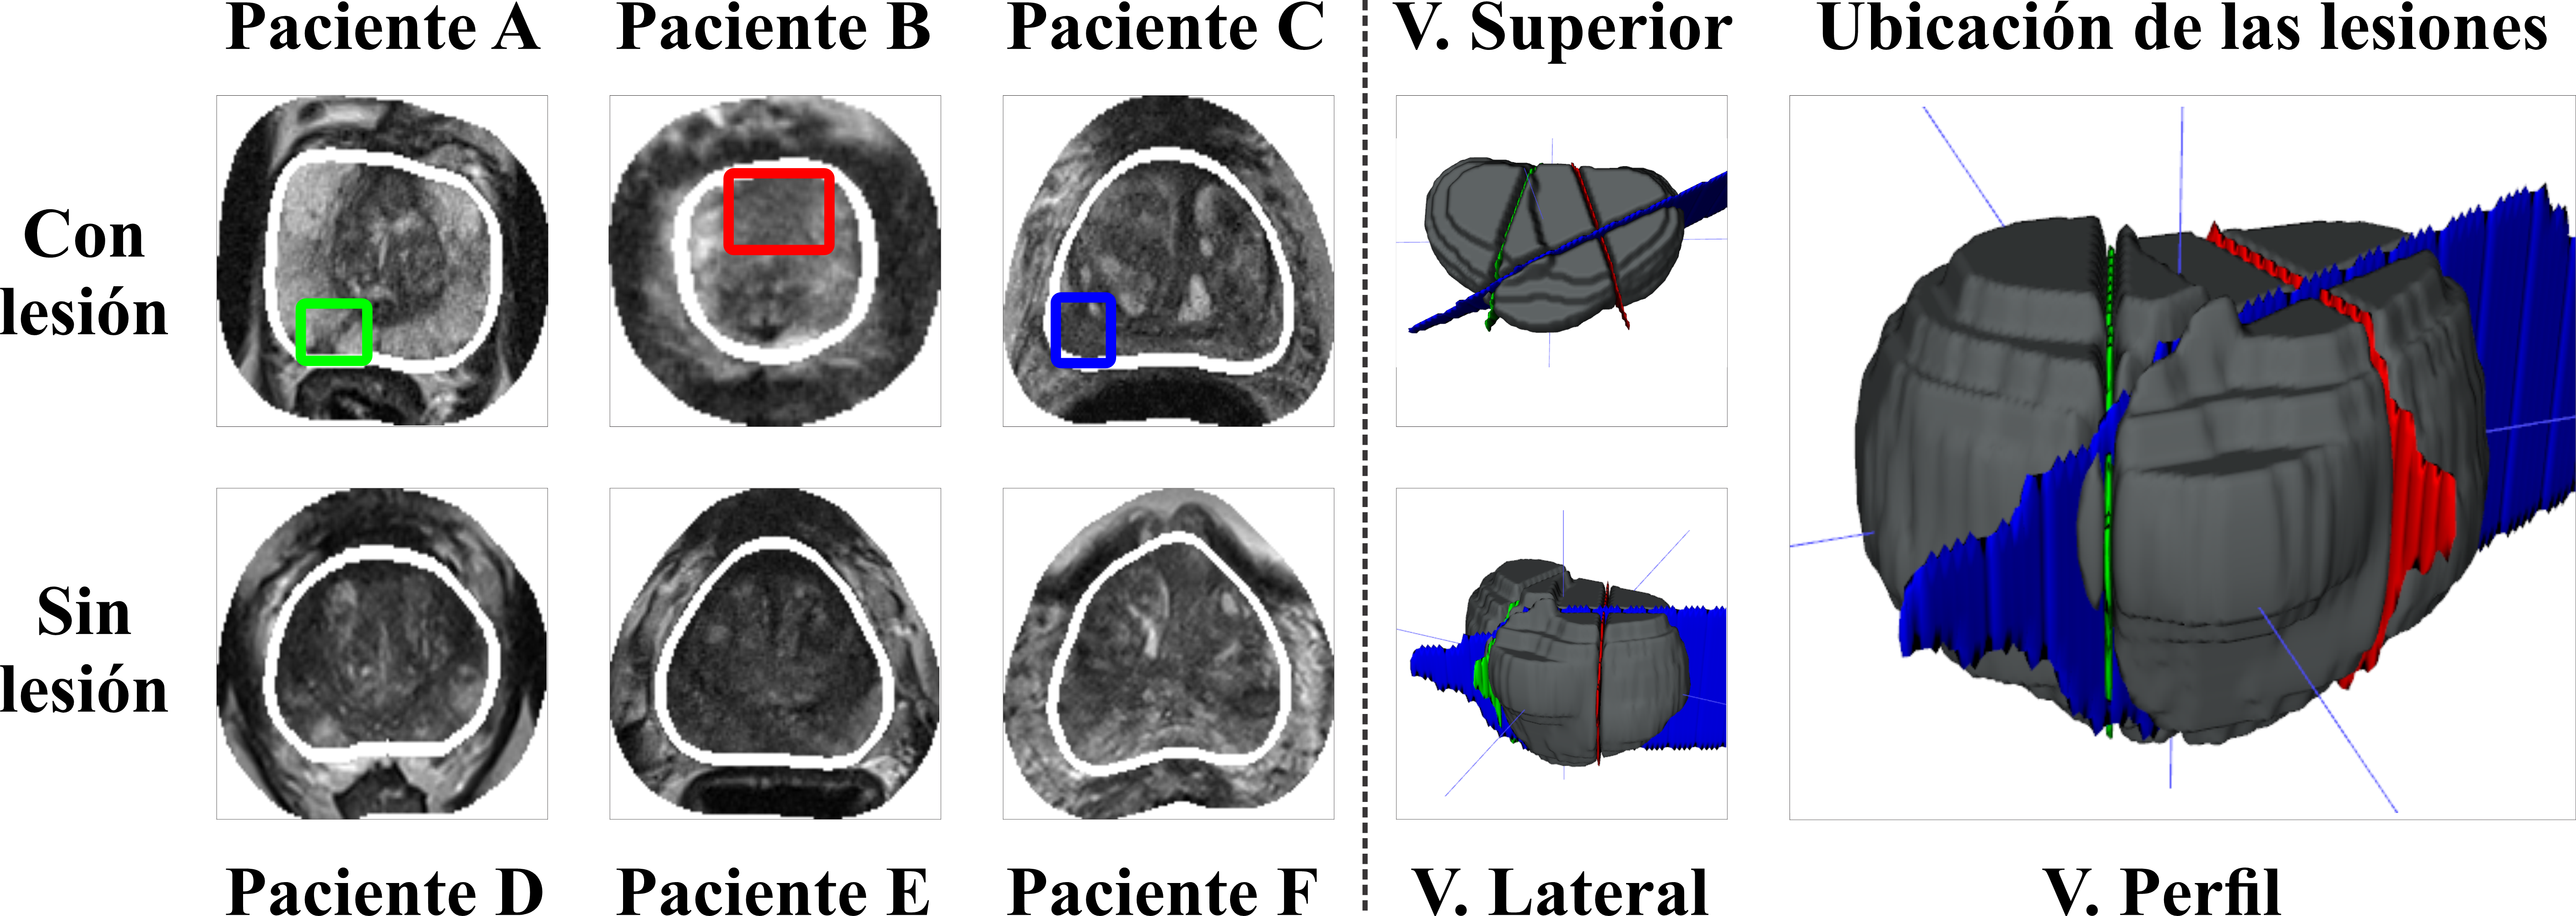
\includegraphics[width=1\textwidth]{imgs/T2WSUMUP.png}
% \caption[Ilustración de lesiones en secuencias T2WI.]{\textbf{Ilustración de lesiones en secuencias T2W.} Imagen construida con el uso de datos bp-MRI de próstata de centros médicos de los Países Bajos \myfootcite{PICAI_BIAS}, y  procesados con el software ITK-SNAP \myfootcite{ITKSNAP}.}
% \label{fig:axT2W}
% \end{figure}

\begin{figure}[h!]
\centering
\caption{Ilustración de lesiones en secuencias T2W.}
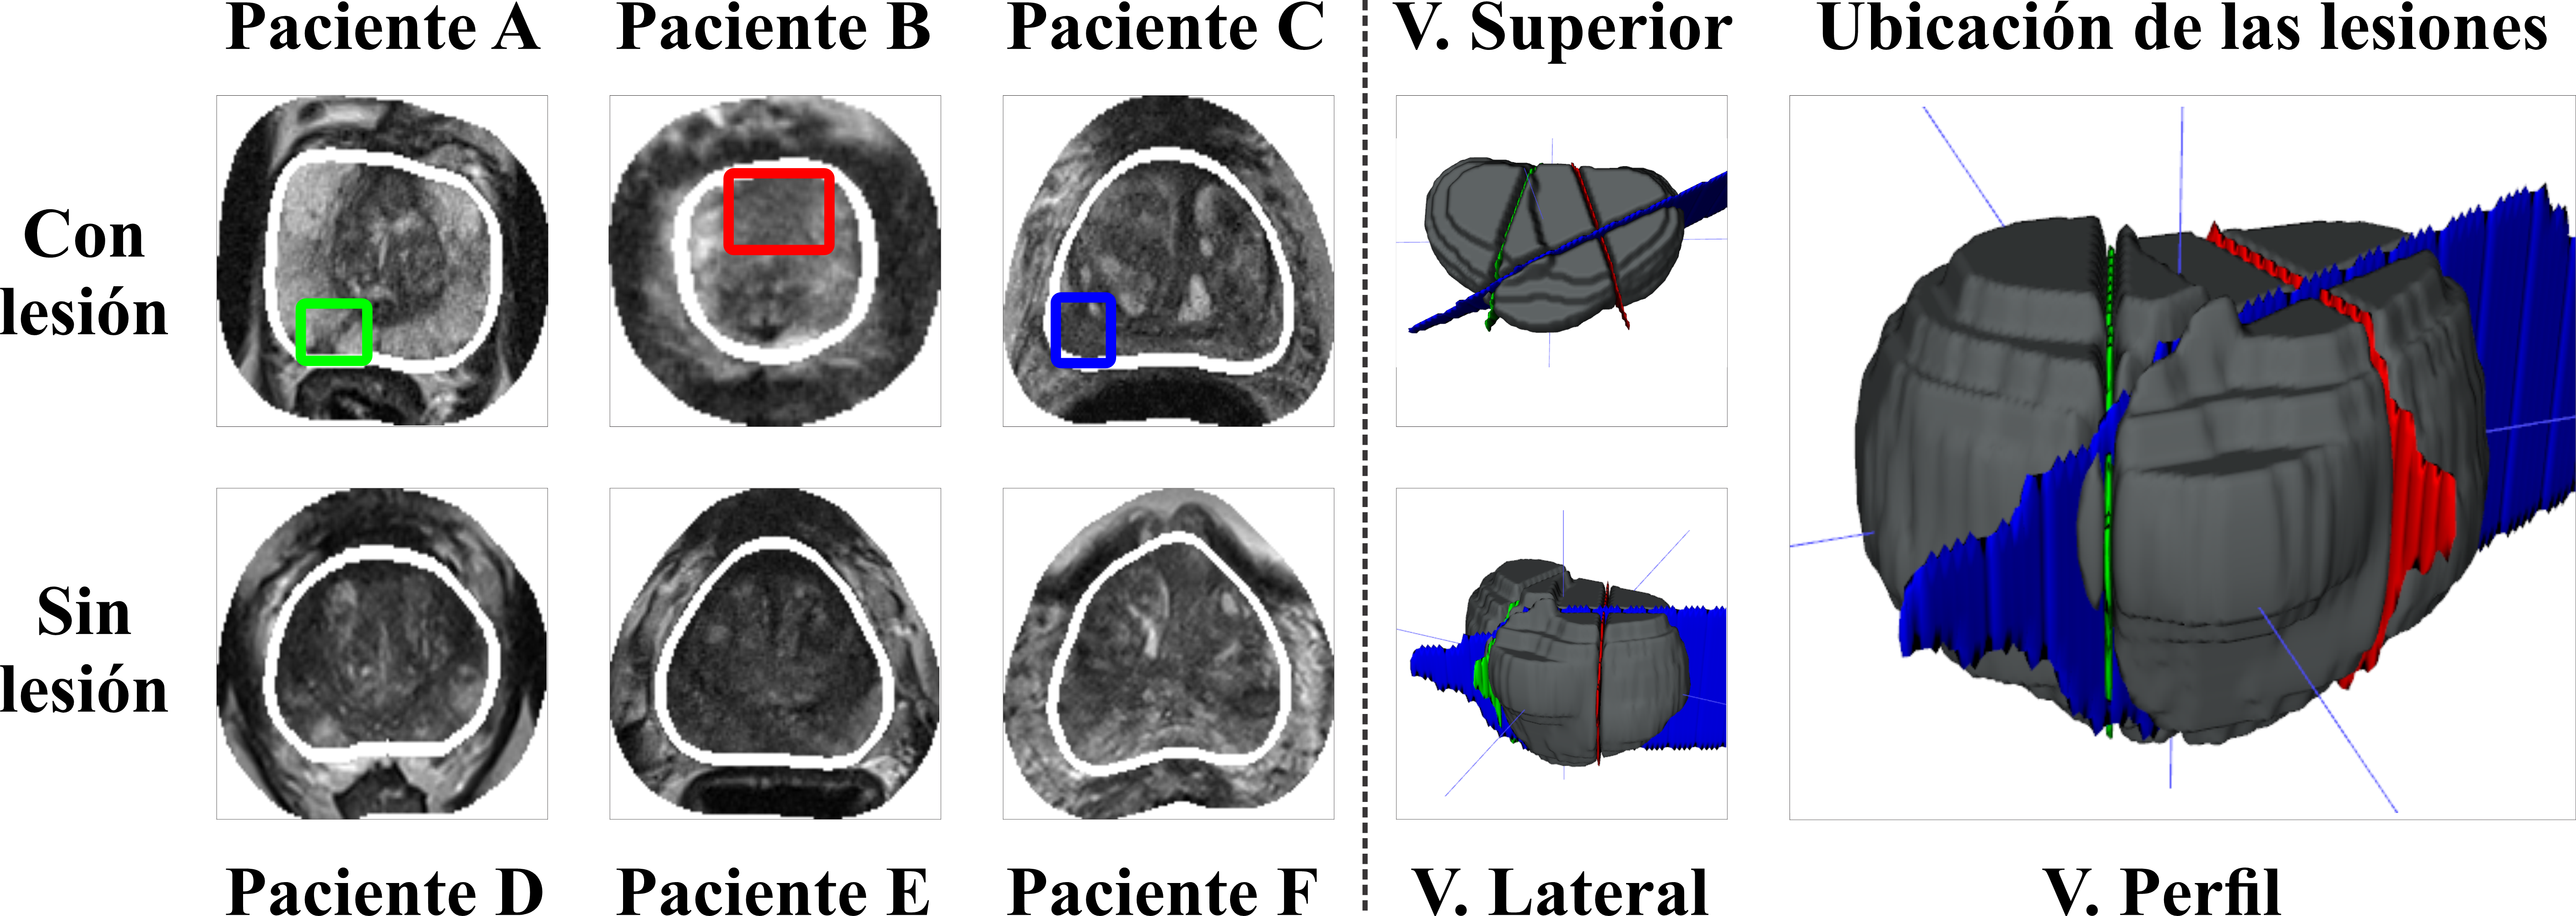
\includegraphics[width=1\textwidth]{imgs/T2WSUMUP.png}
\label{fig:axT2W}
\end{figure}

\begin{figure}[h!]
\noindent \textbf{Nota:} Figura construida con el uso de datos bp-MRI de próstata de centros médicos de los Países Bajos \myfootcite{PICAI_BIAS}, y  procesadas con el software ITK-SNAP \myfootcite{ITKSNAP}.
\end{figure}



\newpage
\subsection{Secuencia de imagen ponderada en difusión (DWI) y mapas ADC. }La secuencia DWI constituye un tipo de imagen que se fundamenta en la movilidad espontánea de las moléculas de agua, conocida como movimiento Browniano \myfootcite{maurer2017diffusion}. Esta secuencia resulta valiosa para obtener información acerca del entorno y los tejidos, debido a que está estrechamente relacionada con las interacciones funcionales del espacio intra y extracelular \myfootcite{Koh2007,Caglic2018}. Característico de esta, es el valor b (b-value), configurable en la adquisición de la secuencia, y connota tiempos y fuerzas de los gradientes que se aplicarán para obtenerla. Convencionalmente, se obtienen secuencias DWI, con diferentes b-value, y es a partir de ellas que se puede llevar a cabo una cuantificación para detectar posibles anormalidades en los tejidos mediante los mapas de Coeficiente de Difusión Aparente (ADC) \myfootcite{lahoti2018role}. Un ADC bajo, que denota un flujo exiguo de agua o difusión reducida, estaría relacionado con tumores o progresiones cancerígenas, que en su mayoría emergen de la producción de biomasa, generando un aumento en la densidad celular y limitando el espacio inter y extracelular disponible. Por el contrario, un flujo desproporcionado podría indicar una degradación celular severa o tejido necrótico \myfootcite{Syer2017,maurer2017diffusion,jacobs2008diffusion}. En la 
%siguientesfiguras (\ref{fig:axDWI}, \ref{fig:axADC}) 
Figura~\ref{fig:axDWI} y Figura~\ref{fig:axADC}
se ilustran cortes de estas secuencias, para diferentes pacientes, además se ilustran casos de glándulas prostáticas con y sin lesión relacionada con el cáncer de próstata. En el panel derecho se muestra una representación volumétrica de la glándula y de los cortes donde se encuentran localizadas las lesiones. 



\begin{figure}[h!]
\centering
\caption{Ilustración de lesiones en secuencias DWI.}
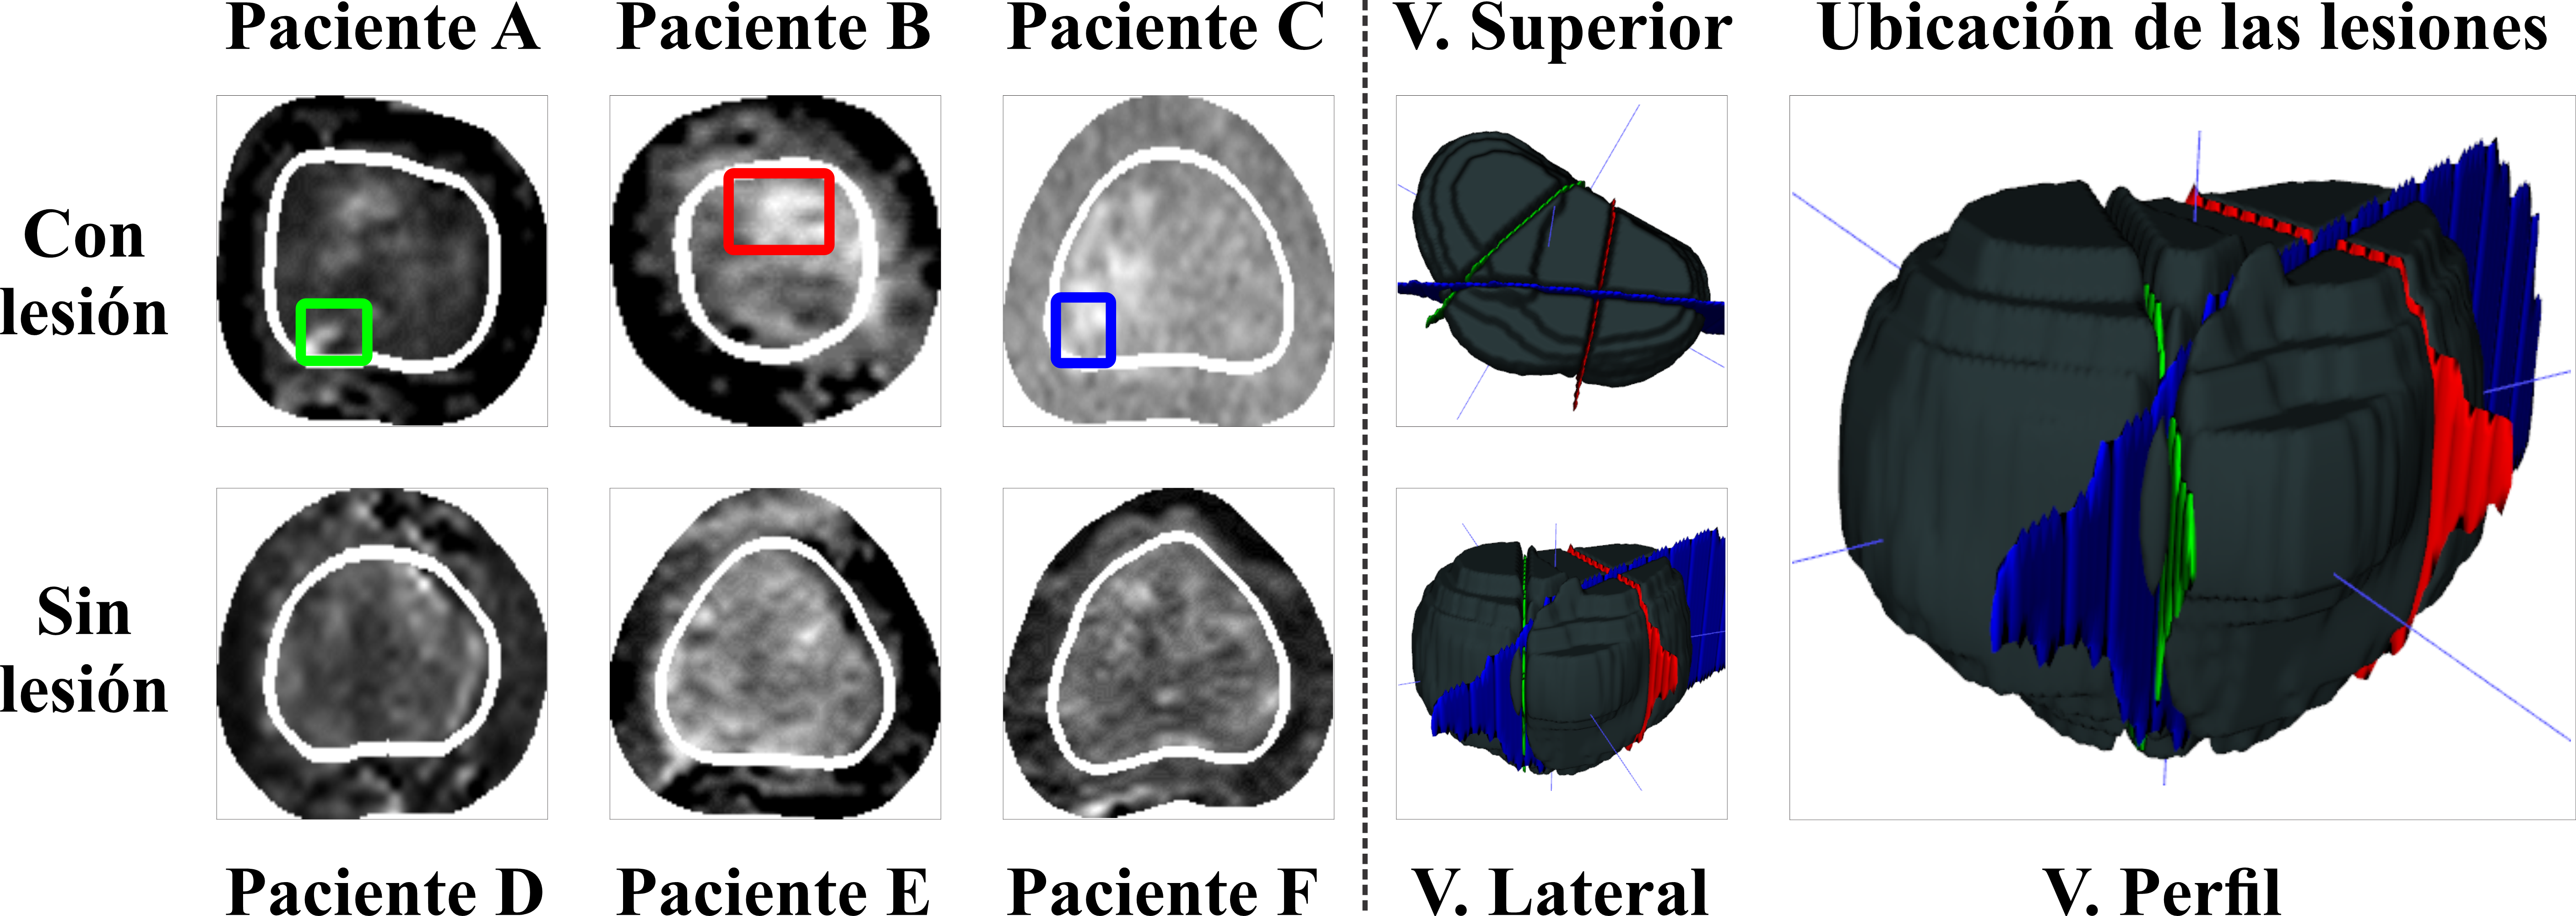
\includegraphics[width=1\textwidth]{imgs/DWISUMUP.png}
\label{fig:axDWI}
\end{figure}

\begin{figure}[h!]
\noindent \textbf{Nota:} Figura construida con el uso de datos bp-MRI de próstata de centros médicos de los Países Bajos \myfootcite{PICAI_BIAS}, y  procesadas con el software ITK-SNAP \myfootcite{ITKSNAP}.
\end{figure}



\begin{figure}[h!]
\centering
\caption{Ilustración de lesiones en secuencias ADC.}
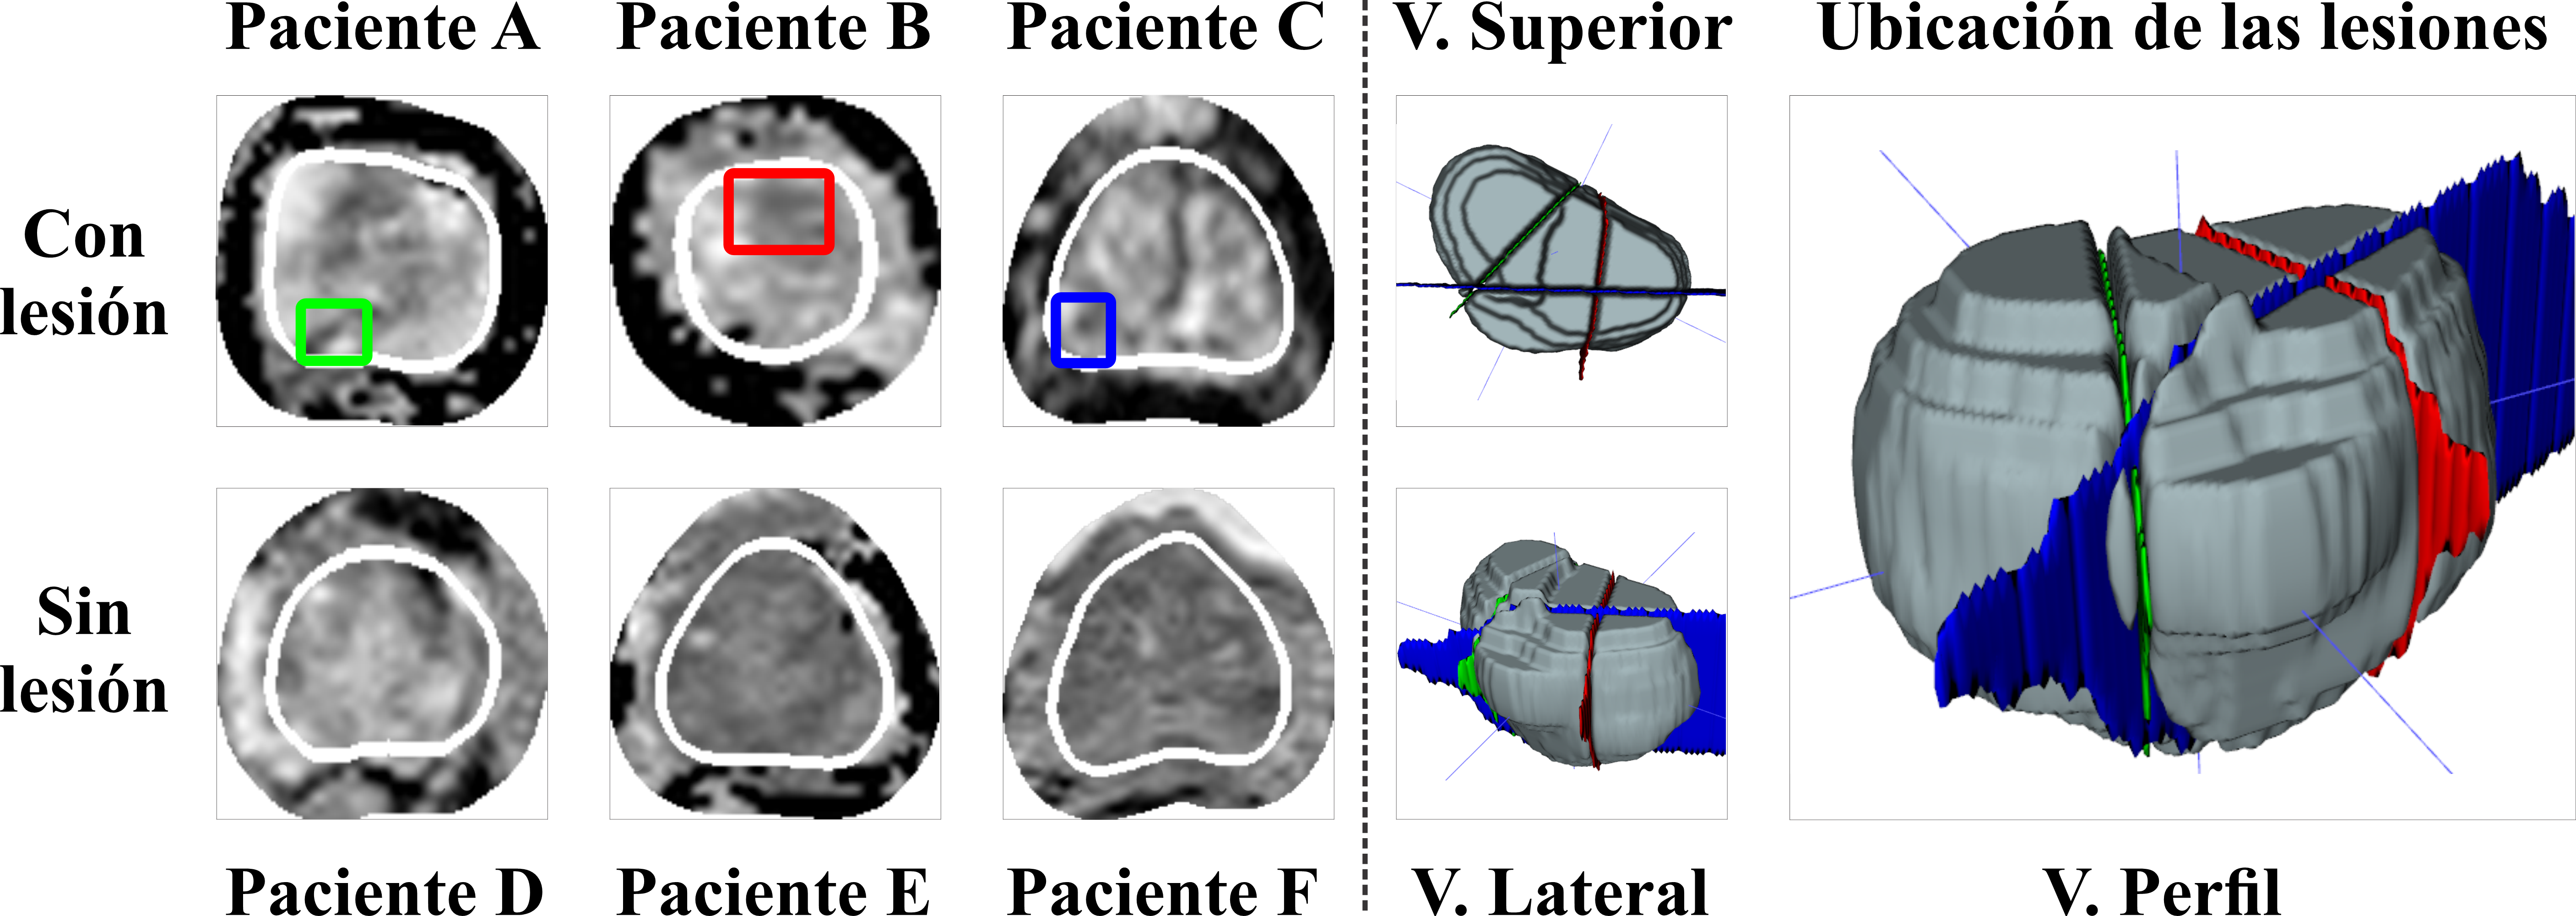
\includegraphics[width=1\textwidth]{imgs/ADCSUMUP.png}
\label{fig:axADC}
\end{figure}

\begin{figure}[h!]
\noindent \textbf{Nota:} Figura construida con el uso de datos bp-MRI de próstata de centros médicos de los Países Bajos \myfootcite{PICAI_BIAS}, y  procesadas con el software ITK-SNAP \myfootcite{ITKSNAP}.
\end{figure}






\newpage
\section{ESTRATEGIAS COMPUTACIONALES DE LOCALIZACIÓN} \label{sec:comp_localiza}
En esta sección se realiza un breve compendio sobre herramientas que se han propuesto para la tarea de localización. 
Para esto, se pueden identificar tres categorías principales en las que se agrupan estos métodos: sistemas de ventana deslizante, sistemas de búsqueda selectiva y sistemas basados en una única observación.

\subsection{Sistemas de ventana deslizante. }% - Haar [25], SIFT [23], HOG [4]
Los sistemas de ventana deslizante son técnicas que fueron ampliamente utilizadas para el procesamiento de imágenes y la detección de objetos de interés. Estos sistemas se basan en la aplicación de un escaneo a diferentes regiones de la imagen, obtenidas mediante el desplazamiento de una ventana o cuadrícula de tamaño fijo a lo largo de la misma. Para mejorar el rendimiento en detección, se ha propuesto extraer características relevantes de las regiones de la ventana, por ejemplo, a través de una muestra local que estime información relevante, y a su vez, escanee cambios en la imagen \myfootcite{DeCroon200797}. Algunos ejemplos de sistemas de ventana deslizante son los basados en las características de Haar wavelet (Haar), Scale-Invariant Feature Transform (SIFT) o Histogram of Oriented Gradients (HOG).\par
Los sistemas basados en Haar propenden por hallar diferencias basadas en la variación de intensidad entre regiones adyacentes de la imagen, con la finalidad de establecer representaciones estructurales, que serán posteriormente procesados por clasificadores como máquinas de soporte vectorial (SVM, por sus siglas en inglés) \myfootcite{Papageorgiou2000}. En la literatura, este método es combinado con un algoritmo de aprendizaje llamado AdaBoost para mejorar la capacidad de discriminación entre objetos y fondos. Esta estrategia es conocida por su eficiencia y mejora en la precisión, por ejemplo, para tareas de detección de objetos \myfootcite{V.Jones}. Por otra parte, el sistema SIFT busca extraer características que sean distintivas e invariantes de las imágenes, aún cuando le son aplicadas transformaciones o quizás distorsiones, como escalamientos, rotaciones, ruido, iluminación y demás cambios de apariencia, esto mediante la asignación de un descriptor basado en el gradiente local. El método es ampliamente utilizado para el reconocimiento de objetos y ha demostrado ser efectivo incluso en escenarios con problemas de oclusión, logrando además, un rendimiento casi de tiempo real \myfootcite{Lowe2004}. Finalmente, los sistemas basados en HOG utilizan distribuciones probabilísticas de los gradientes locales en diferentes regiones de la imagen para de esta forma capturar de mejor manera características invariantes. Posteriormente, estas distribuciones alcanzadas son utilizadas para entrenar un clasificador lineal como SVM. \myfootcite{Dalal-Hog}. Algunas de estas metodologías han sido utilizadas para recalar en la localización y detección de lesiones prostáticas en MRI \myfootcite{Qian2016,Lay2017}.

% A pesar de su utilidad, los sistemas de ventana deslizante presentaron algunos desafíos. Por ejemplo, requieren evaluar muchas regiones candidatas, lo que puede ser computacionalmente costoso, además pueden producir múltiples detecciones del mismo objeto, lo que requiere mecanismos, no siempre efectivos para tratar redundancias, así mismo, pueden tener dificultades para adaptarse a variaciones en la forma, pose u oclusión del objeto, lo que afecta su robustez, eficacia o representatividad del aprendizaje.




\subsection{Sistemas de búsqueda selectiva. }Con el antecedente de las redes convolucionales (CNN), los sistemas de búsqueda selectiva afloran como una propuesta para generar conjuntos de regiones candidatas, que puedan contener objetos, para una ulterior clasificación. Por ejemplo, el algoritmo \textit{Regions with CNN features} (R-CNN) para la detección de objetos, combina la postulación de regiones con las características extraídas por una red neuronal convolucional (CNN).
% Este algoritmo demostró significativas mejoras en precisión, su funcionamiento se estructura en tres etapas.
Propiamente, este algoritmo genera propuestas de regiones por imagen, luego extrae un vector de características que se proyecta a un clasificador \myfootcite{Girshick2014}. La R-CNN cuenta con diferentes actualizaciones y mejoras entre las que se enmarca la Fast R-CNN, la Faster R-CNN y la Mask R-CNN \myfootcite{RCNNfamily}. \par La primera, Fast R-CNN, postula una red que se encarga del proceso de proponer regiones, haciéndolo de manera más eficiente. Esta red también se reconoce por la introducción del concepto Region of Interest (RoI) Pooling, empleado para proyectar las regiones candidatas sobre los mapas de características de la CNN \myfootcite{GiFast}. En consideración, la Faster R-CNN basa su detección en la Fast R-CNN, agregando una red de propuestas de regiones (RPN, region proposal network), que dispensa del algoritmo de búsqueda selectiva. Además, realiza la tarea directamente desde el mapa de características de la CNN, acelera el proceso de detección, se destaca que comparten características convolucionales con la red de detección \myfootcite{RenFaster}. Por otra parte, fue introducida la Mask R-CNN, que adiciona un proceso de segmentación semántica, donde se añade una rama paralela que genera una máscara binaria para cada región candidata. De esta forma, Mask R-CNN puede producir no solo la clase y la caja delimitadora del objeto, sino también una delineación del contorno del objeto  \myfootcite{heMask}. Estas arquitecturas en relación al cáncer de próstata han sido integradas en etapas de preprocesamiento \myfootcite{Soni2022,Dai2021,Liu2019}.


\subsection{Sistemas basados en una única observación. }Los sistemas de detección de objetos en imágenes basados en una única observación son una aplicación innovadora que abrió nuevas perspectivas en el campo de visión por computador. Algunos de los sistemas que operan bajo este concepto incluyen You Only Look Once (YOLO) \myfootcite{RedYolo}, Single Shot MultiBox Detector (SSD) \myfootcite{LiuSSD}, RetinaNet \myfootcite{LinRetin}, SpineNet \myfootcite{DuSpine} y DEtection TRansformer (DETR) \myfootcite{CarionDetr}. \par

A diferencia de los algoritmos de sistema de búsqueda selectiva, estos algoritmos realizan la detección de objetos en una sola pasada a través de la red neuronal y utilizan diferentes estrategias para mejorar la precisión y el equilibrio entre las clases de objetos. Por ejemplo, la estrategia YOLO es una técnica de detección de objetos en tiempo real que propone dividir la imagen en una cuadrícula de celdas, sobre las cuales se ejecutarán tareas de detección. Para esto, en cada celda son propuestos unos cuadro delimitadores, a los cuales, durante el entrenamiento se les asigna puntuaciones, en referencia a la confianza y precisión por la existencia de un objeto de cierta clase en dicho cuadro delimitador. La red ajusta también la ubicación y el tamaño de los cuadros delimitadores, maximizando su precisión de forma que se seleccione el cuadro más confiable. Específicamente, la red YOLO involucra una función de pérdida que tiene en cuenta varios factores: la precisión de la localización del cuadro delimitador, la confianza de la detección y la precisión de la clasificación de objetos. Su uso se ha extendio a tareas como la vigilancia, la conducción autónoma, incluso el reconocimiento de imágenes \myfootcite{RedYolo}. Por su parte, Single Shot MultiBox Detector (SSD) es una propuesta para detección en tiempo real, que a diferencia de la YOLO, busca simplificar y ser mas eficiente en el proceso de selección de los cuadros delimitadores. Esto lo logra mediante un enfoque multi-escala, el cual mejora la detección de objetos de diferentes tamaños al hacer el análisis de cajas delimitadoras sobre características de diferente resolución. De manera similar a la YOLO, la red genera puntuaciones para la presencia de cada categoría de objeto en cada caja delimitadora. Además, se combinan las predicciones de los múltiples mapas de características, incluyendo así una detección mas robusta que trate con diferentes tamaños de objeto \myfootcite{LiuSSD}. Sin embargo, esta robustez de las características alcanzadas en esta red, dependen de los cuadro delimitadores definidos desde un inicio. A partir de esto, surge RetinaNet, una red para detección de objetos que se compone de una CNN  de tipo ResNet, y cuya principal contribución se centra en la introducción de una Feature Pyramid Network (FPN). FPN toma características profundas y crea una piramide de caracteristicas a diferente grado de resolución. Seguidamente, se utilizan dos subredes: una de clasificación para los niveles de la FPN, regida por una pérdida focal que soporta el problema de desbalance de clases en imágenes con mucho fondo, esto asignando un mayor peso a las cajas delimitadoras que contienen objetos difíciles de detectar o poco frecuentes; y una segunda red dedicada a la predicción a través de regresión, de los centros y áreas de las cajas delimitadoras. Los experimentos muestran que la RetinaNet, con la pérdida focal propuesta, supera a los detectores que la anteceden \myfootcite{LinRetin}. 
En vía de crear una mejor fusión de características multi-escala, el equipo de Google propuso la SpineNet. Esta propuesta identifica como un problema para la tarea de localización y detección, la captura de características a través de una reducción espacial, como lo hace el método involucrado en la FPN. Por el contrario, introducen un método más eficaz con un backbone dinámico, donde los mapas de características se proyectan a través de conexiones entre diferentes escalas. Para esto, la SpineNet utiliza técnicas de diseño automático de arquitectura (NAS, por sus siglas en ingles \textit{Neural Architecture Search}). Como resultado, demuestran que esta estrategia permite capturar mejor la información espacial y fusionar mejor la información, dos aspectos claves en tareas de detección \myfootcite{DuSpine}. Por último, se han propuesto recientemente redes que involucran mecanismos de atención mediante la introducción de arquitecturas \textit{Transformer} en el codificador extractor de características y generador de las cuadros candidatos. Este tipo de estrategias permiten refinar las predicciones de las clases y las ubicaciones de los cuadros, utilizando incluso varias redes de atención de múltiples cabezas \myfootcite{CarionDetr}. Estos enfoques han sido aproximados para el cáncer de próstata en \myfootcite{Salman2022,Seetharaman2021}.



\section{ANTECEDENTES LOCALIZACIÓN DE LESIONES CS-PCA}\label{sec:localiza_pca}Para el personal médico radiológico el diagnóstico de lesiones csPCA en imagenología MRI es una tarea compleja que requiere una amplia experticia, y aún teniéndola, persiste gran variabilidad de interpretación dependiendo del lector \myfootcite{Twilt2021}. El desarrollo de herramientas diagnósticas basadas en computador (CAD, Computer aided diagnosis), y en especial aquellas apoyadas por inteligencia artificial, resultan entonces fundamentales para soportar la detección de lesiones anormales y su correspondiente diagnóstico \myfootcite{Mata2021,Harmon2019}. Para el caso del soporte a labores urológicas, estas herramientas pueden mejorar la especificidad y la eficiencia del experto radiólogo, en especial cuando existen lesiones en zonas difíciles de interpretar, como sucede en lesiones ubicadas en la zona transicional de la próstata \myfootcite{murphy2013expanding}. A razón de ello, estas herramientas pueden contribuir a la reducción de variabilidad inter-lector \myfootcite{Gaur2018}. En los protocolos clínicos existen acuerdos y protocolos clínicos que establecen la importancia de utilizar los diferentes parámetros MRI, por la significancia que cada una de ellas brinda para la localización y diagnóstico final \myfootcite{Scott2021,maurer2017diffusion,Wu2019}. Es por esto, que las herramientas propuestas deben tener en primer lugar la capacidad de capturar, ubicar y cuantificar patrones radiómicos de importancia, con la finalidad de obtener herramientas óptimas que permitan posteriormente una evaluación final por parte del lector \myfootcite{Algohary2018}. Por consiguiente, se introducirán a continuación herramientas de localización y detección propuestas a la fecha.\par

Una primera aproximación común para esta tarea en imágenes MRI de próstata ha sido el análisis por regiones. En ese sentido, (Qian et al., 2016) propuso un framework que involucraba una interpretación de todas las regiones de la próstata mediante el análisis del contexto en las estructuras de los tejidos \myfootcite{Qian2016}. Por su parte, en \myfootcite{Lay2017}, se incorporó la ponderación de instancias para evitar sesgos con el volúmen de cada lesión, así como el uso de delineaciones manuales de la próstata.  Aunque estos dos métodos obtienen buenos resultados, sus estudios fueron realizados con una limitada cantidad de datos, afectando posiblemente su capacidad de generalización y representación. Además, el enfoque de estos se basa en los primeros sistemas de localización de ventana deslizante y clasificadores como bosques de decisión (DTs) y SVM, no especializados en la extracción de características de la imagen para la tarea de localización. Para esto, posteriormente se postularon redes de extremo a extremo que vinculan dos subredes para las tareas de registro y detección mediante la introducción de CNNs \myfootcite{Le2017,Wang2018}. A pesar de alcanzar buenos resultados en cuanto a sensibilidad y especificidad, el primero enuncia valores bajos de especificidad, que podría inducir errores, hasta someter pacientes a tratamientos innecesarios, mientras el segundo muestra una baja sensibilidad, que podría desestimar pacientes con lesiones significativas que requieran atención y tratamiento. A partir de esto, otros trabajos propusieron enfoques similares, destinando redes CNN extremo a extremo en sus desarrollos \myfootcite{Ishioka2018,Sumathipala2018,Cao2019}. Así mismo, se han propuesto trabajos que buscan alcanzar una mejor localización utilizando información mapeada desde imágenes histopatológicas \myfootcite{Dai2021,Seetharaman2021}, inclusive, autores como (Salman et al., 2022) han propuesto el uso de la herramienta YOLO, para maniobrar la localización del cáncer de próstata \myfootcite{Salman2022}. Sin embargo, estos enfoques involucran el registro de imágenes MRI e histopatológicas, lo cual puede carecer de una buena congruencia y verse afectado por una mala correspondencia entre las imágenes. Por otra parte, la evolución de diferentes estrategias en CNNs ha permitido que emerjan nuevos métodos, por ejemplo, involucrando módulos residuales, utilizando transfer learning, e incluso, incluyendo mecanismos de atención para segmentación \myfootcite{Xu2019,Abbasi2020,Mehralivand2020}. 
% , mas, sus desarrollos se basaron también en datos monocentro. Por otra parte, también se han involucrado 
No obstante, este último enfoque no alcanza resultados satisfactorios, sugieren que es necesario un conjunto de datos óptimos con buen procesamiento, e incluso que incluya estudios de diferentes centros para capturar mejor la alta variabilidad que concierne a las lesiones prostáticas en MRI \myfootcite{Mehralivand2020}. Además, explicitan que tareas de clasificación de lesiones no parecerían muy adecuadas, pues es ciertamente subjetiva y dificulta la tarea de segmentar la lesión.
Enfoques similares de segmentación, como los modelos Panópticos \myfootcite{Xu2019}, donde metodología semántica y segmentación de instacias fueron involucradas, arrojaron mejoras en el rendimiento de detección. 
De la misma manera, existen abordajes 3D, donde buscan enfocarse en características relevantes en múltiples resoluciones a través de mecanismos de atención y CNNS 3D \myfootcite{Saha2021}, así mismo, involucran información de dominio clínico para sus desarrollos. También, los autores resaltan la importancia de diversificar en herramientas CAD que resulten menos dependientes a los conjuntos de datos. Recientemente, se han decantado por aproximarse a soluciones retomando métodos de KNN, donde se refieren a  matrices de concurrencia, o reducción de ruidos por transformaciones, hasta clasificadores tradicionales \myfootcite{Anand2023}. Sin embargo, es claro que estructuras especializadas en imágenes han mostrado ser más eficientes. Otras soluciones involucran esquemas adversarios-generativos (Gans, por sus siglas en Inglés) \myfootcite{Patsanis2023}. No obstante, su propuesta desestiman las características radiómicas variopintas al no involucrar secuencias anatómicas y funcionales MRI, donde en la práctica médica, y además, en bpMRI, ninguna es sustitutoria.\par De esta manera, es evidente que, aunque los desarrollos relacionados con la detección de lesiones CsPCA son importantes, su enfoque propositivo de frameworks propios y esfuerzos en tareas de clasificación, podrían llevar a un descuido o desaprovechamiento de las herramientas de localización que conforman el estado del arte, las cuales han sido probadas y validadas por la comunidad académica y han demostrado ser efectivas y confiables.\pagebreak
 % Parkinsonian oculomotor analysis


\chapter{PROBLEMA DE INVESTIGACIÓN}

El cáncer de próstata es una enfermedad que afecta a un gran número de hombres en todo el mundo y su detección temprana es crucial para reducir la agresividad y la cantidad de muertes asociadas. Aunque el estudio de lesiones prostáticas mediante resonancia magnética biparamétrica (bp-MRI) es un criterio estándar para la detección y diagnóstico del cáncer de próstata, la localización de estas lesiones sigue siendo subjetiva a la experticia del radiólogo y su caracterización reporta bajos niveles de sensibilidad. Además, hay diferencias notables entre el diagnóstico por parte de diferentes expertos. Lo cual ha ampliado la necesidad de personal con amplia experiencia, lo que resulta insuficiente para satisfacer la alta demanda de pacientes. Por lo tanto, resulta crucial el desarrollo de herramientas computacionales que permitan la localización automática, precisa y eficiente de lesiones prostáticas. En particular, resulta relevante la implementación de una herramienta basada en aprendizaje profundo que especialice la tarea de localización, para servir de soporte y mejorar el diagnóstico del cáncer de próstata clínicamente significativo csPCA en estudios de bp-MRI.



 % Research Problem  
    \chapter{OBJETIVOS}

\section*{Objetivo General}

\begin{itemize}
Desarrollar una estrategia de aprendizaje profundo para la localización de regiones clínicamente significativas de cáncer de próstata (csPCa) en secuencias multimodales MRI biparamétricas (bp-MRI).
\end{itemize}


\subsection*{Objetivo Específicos}
\begin{itemize}
\item \textcolor{black}{Acondicionar un conjunto de datos con estudios que incluyan al menos dos secuencias MRI de la glándula prostática junto con sus respectivas anotaciones por expertos radiólogos.}
\item \textcolor{black}{Adaptar una arquitectura de aprendizaje profundo para llevar a cabo la localización de lesiones prostáticas clínicamente significativas desde secuencias bp-MRI.}
\item \textcolor{black}{Implementar una estrategia de entrenamiento para la localización de lesiones prostáticas clínicamente significativas en secuencias bp-MRI.}
\item \textcolor{black}{Evaluar el desempeño de la estrategia propuesta en cuanto a la capacidad de localizar lesiones prostáticas clínicamente significativas.}
\end{itemize}
 %Objectives
\chapter{MÉTODO PROPUESTO}


\section{Conjunto de datos de lesiones de Próstata}

Para el desarrollo de este trabajo, se consideró la cohorte de datos de entrenamiento y desarrollo público \cite{Picai_dataset} contenida en el conglomerado PI-CAI (Prostate Imaging: Cancer AI) \cite{PICAI_BIAS}. Este conjunto de datos es relevante por ser multicentro y multi-equipo. Las secuencias se capturaron en tres centros médicos de los Países Bajos: \textit{Radboud University Medical Center} (RUMC), \textit{Ziekenhuis Groep Twente} (ZGT), \textit{University Medical Center Groningen} (UMCG), en equipos de fabricantes Siemens Healthineers o Philips Medical Systems, con diferentes intensidades de campo (1.5T o 3T). Es longitudinal en el tiempo, con casos de estudio fechados entre 2012 y 2021; homogéneo en sus protocolos, la adquisición se siguió a detalle con lo indicado en el protocolo de imagenología \cite{Engels2020}; e interdisciplinar, en su diseño se contó con un consejo asesor científico internacional compuesto por dieciséis expertos en IA de próstata, radiología y urología.

De la misma manera, estos estudios de resonancia bp-mRI cuentan con las respectivas anotaciones de lesión. Esto implica una segmentación a nivel de vóxel que demarca zonas específicas o regiones dentro de la glándula prostática o en el tejido circundante, así como una posible graduación de la lesión. Estas tareas son realizadas por un profesional capacitado con más de 20 años de experiencia, o un residente bajo la supervisión de un radiólogo. Para lo anterior, se basan en el protocolo de anotación PI-RADS (Prostate Imaging Reporting and Data System), siguiendo las instrucciones de su última versión, la 2.1 \cite{Scott2021}. Por otra parte, es importante mencionar el protocolo ISUP (Histopathological grading of prostate cancer). Aunque ambos protocolos buscan la determinación y estratificación de una lesión prostática y trabajan en el mismo rango [1,5], esto no significa que sean comparables. El protocolo ISUP se destina al reporte únicamente de componentes histológicos, que están en etapas subsecuentes del protocolo de atención; no así las radiológicas que son las establecidas para atención inicial y screening poblacional. Es decir, en este conjunto de datos, los \textit{ground truths} de las lesiones, aunque en un primer momento están determinadas por el radiólogo, se han verificado con el segundo protocolo para confirmar su naturaleza. De acuerdo a lo anterior, se estableció que son casos de estudio positivos aquellos confirmados histológicamente con la denominación ISUP>=2, y negativos aquellos con ISUP <=1 o cuya bm-MRI se haya determinado <=2 y no tengan seguimiento.

En ese sentido, PI-CAI (Prostate Imaging: Cancer AI), cuenta con un total de 1,500 casos de estudio, donde se incluyen además casos del denominado PROSTATEx \cite{Prostatex}, un conjunto precedente de similares características. De todos los casos de estudio, 425 son los que han sido determinados como positivos, con lesión csPCA, pero únicamente 220 son aquellos que están provistos de una marcación asociada, según el estándar ya comentado.


%The MRI sequences were pre-processed following the steps provided by the PI-CAI challenge \cite{saha-picai}. This involved resampling each MRI sequences to a voxel spatial resolution of $0.5 \si{mm} \times 0.5 \si{mm} \times 3.0 \si{mm}$, and then cropping around the center of the scan to obtain a study with 24 slices, each one with size $384 \times 384$. Thereafter, each independent sequence T2, ADC, and DWI were normalized using a min-max normalization to range the values in the interval $[0,1]$.

% In this work, a patch-based approach was followed to create the regions of interest for classification. For this, a volumetric region of interest (vROI) was extracted for each BP-MRI sequence (T2, ADC and DWI) of each case, by centering on the expert annotation with a fixed size of $12 \times 32 \times 32$, where $32\times 32$ are the spatial dimensions in the transverse plane (where $x$ denotes the frontal axis and $y$ the sagittal axis), and $12$ the number of slices, corresponds to the spatial dimension along the vertical axis, denoted by $d$. The respective vROIs are referred to as $\mathbf{X}_{T2}, \mathbf{X}_{ADC}$ and $\mathbf{X}_{DWI}$. For no-csPCa studies, a slice $i_d$ between slices 9 and 15 (included), and a random point at location $(i_x, i_y)$ in the prostate gland on the slice $i_d$ were randomly selected.
% For this, AI-derived delineations of the prostate gland provided by the challenge were used \cite{bosma-ai-delineations}. The vROI was extracted thereafter around the same location $(i_d,i_x, i_y)$ on each sequence $\mathbf{X}_{T2}$, $\mathbf{X}_{ADC}$ and $\mathbf{X}_{DWI}$, see Figure~\ref{fig:vROIS}.

\section{Procesamiento de datos}

En el contexto de este estudio, cada secuencia de los casos de estudio fue sometida a un proceso de preprocesamiento. Para esto, se utilizaron herramientas estandarizadas proporcionadas por el pipeline general descrito en \cite{PICAI_challenge}. Inicialmente, se aplicaron ciertos remuestreos a algunas propiedades de las imágenes; Entre ellos, se modificó el espaciado de los vóxeles a 0.5, 0.5, 3.0 mm y se estableció un tamaño espacial de matriz de 384x384x24. Además, para el nuevo tamaño de imagen, se tuvo en cuenta  centrarse en la glándula prostática. Posteriormente, se alineó cada una de las secuencias contenidas en los casos de estudio con su secuencia principal establecida, en este caso la T2W.  Por otra parte, se tuvo en cuenta la información de metadatos de cada secuencia para alinear las posibles discrepancias en los vóxeles. Finalmente, se verificó que no existieran errores posibles durante el remuestreo para las anotaciones. Esto incluye, por ejemplo, verificar que la conectividad de las lesiones entre slices no haya sido modificada o que el número de lesiones csPCa no discrepe.

Consecuentemente, en el proceso de preparación de los datos para el entrenamiento del modelo, se examinó a nivel de slice cada secuencia de los casos estudio, para identificar aquellos con región csPCA. Al margen de lo anterior, nos valimos de una segmentación apta, exclusiva de la glándula prostática, referida por el algortimo\cite{PICAI_challenge}, entrenado mediante anotaciónes de glándulas prostáticas de \cite{Prostatex_Annotations}. La finalidad del uso de estas segmentaciones es concurrir en áreas prostáticas de interés, mucho más centradas en el órgano, eliminando el ruido de fondo o artefactos.

El procedimiento se sigue así: para los slices donde se correlacionaba una anotación de glándula se establecía un cuadro delimitador de 150 x 150 píxeles, manteniendo el centro glandular constante, proporcionando así un contexto más amplio y garantizando posibles lesiones muy periféricas. 

Por lo demás, estas áreas extraídas se utilizaron como máscaras de recorte y se aplicaron tanto a los slices caso de estudio bpMRI, así como a las anotaciones de lesión. Estas nuevas áreas de los slices de cada secuencia se normalizaron y se combinaron para formar una imagen RGB, es decir, se involucró cada secuencia (T2W, HBV Y ADC) en un canal en la imagen resultante. Estas imágenes RGB son las que contituyen el dataset final de entrenamiento.

En cuanto a las anotaciones de lesión csPCA, indicadas por radiología, se realizó un aumento del 30\% del cuadro que delimita la lesión csPCA marcada por el radiólogo, manteniendo el centro constante, normalizando las coordenadas del cuadro delimitador. Adicionalmente, se llevó a cabo un mapeo de estos cuadros delimitadores csPCA, en el formato [Presencia de lesión, coordenada\_X, Coordenada\_Y, Alto,  Ancho]. Este formato de las anotaciones clarifica de mejor manera las ubicaciones o áreas de interés csPCA, asegurando que se cuente con la información más relevante para la utilización en modelos de localización. 


\section{Red de localización de lesiones significativas de cáncer de Próstata}


% ---> 1 parrafo de resumen muy breve de la arquitectura o los metodologicos que su sigue su red desde la entrada hasta la prediccion ... "En la fgura XX esta el pielene..."


La red propuesta para la localización de lesiones significativas de cáncer de próstata (csPCA) se basa en la arquitectura YOLOv5 y sigue una metodología de tres etapas: extracción de características, cuello y cabeza.

En la etapa de extracción de características, se procesa la imagen de entrada para obtener mapas de características de alto nivel. Estos mapas son representaciones de la imagen original que capturan detalles como bordes, texturas y patrones. Estos detalles son cruciales para la identificación de lesiones csPCA. A medida que la imagen se reduce en tamaño, el número de canales de los mapas de características aumenta. Esto permite a la red aprender y representar diferentes granularidades de las lesiones, lo que ayuda en la generalización y en el manejo de la heterogeneidad inherente de las lesiones.

La etapa del cuello implementa estrategias de PANET para realizar submuestreos estratégicos. Esto permite a la red trabajar con diferentes resoluciones y garantiza que los mapas de características tengan un buen valor semántico. Además, se utiliza el arquetipo SPPF (Spatial Pyramid Pooling Fusion), que mejora la funcionalidad del campo receptivo y permite una mayor fluidez en la red. El campo receptivo se refiere a la región en la imagen de entrada que una neurona particular puede “ver”. Al aumentar el campo receptivo, la red puede capturar detalles a diferentes escalas, lo que es crucial para la detección de lesiones de diferentes tamaños.

Finalmente, en la etapa de la cabeza, la red genera las predicciones de localización, existencia y categoría de las lesiones csPCA a partir de los resultados de las etapas anteriores. Esto se realiza mediante capas completamente conectadas (fully connected), que también realizan cálculos para el ajuste correcto de las localizaciones de los cuadros delimitadores. Estas capas predicen la localización, la existencia y la categoría del objeto (en este caso, las lesiones csPCA).

En la Figura (\ref{fig:pipeline}) se puede observar el pipeline completo de la red.



\begin{figure}[h!]
	\centering
	\caption{Pipeline General para la localización de lesiones csPCA}
	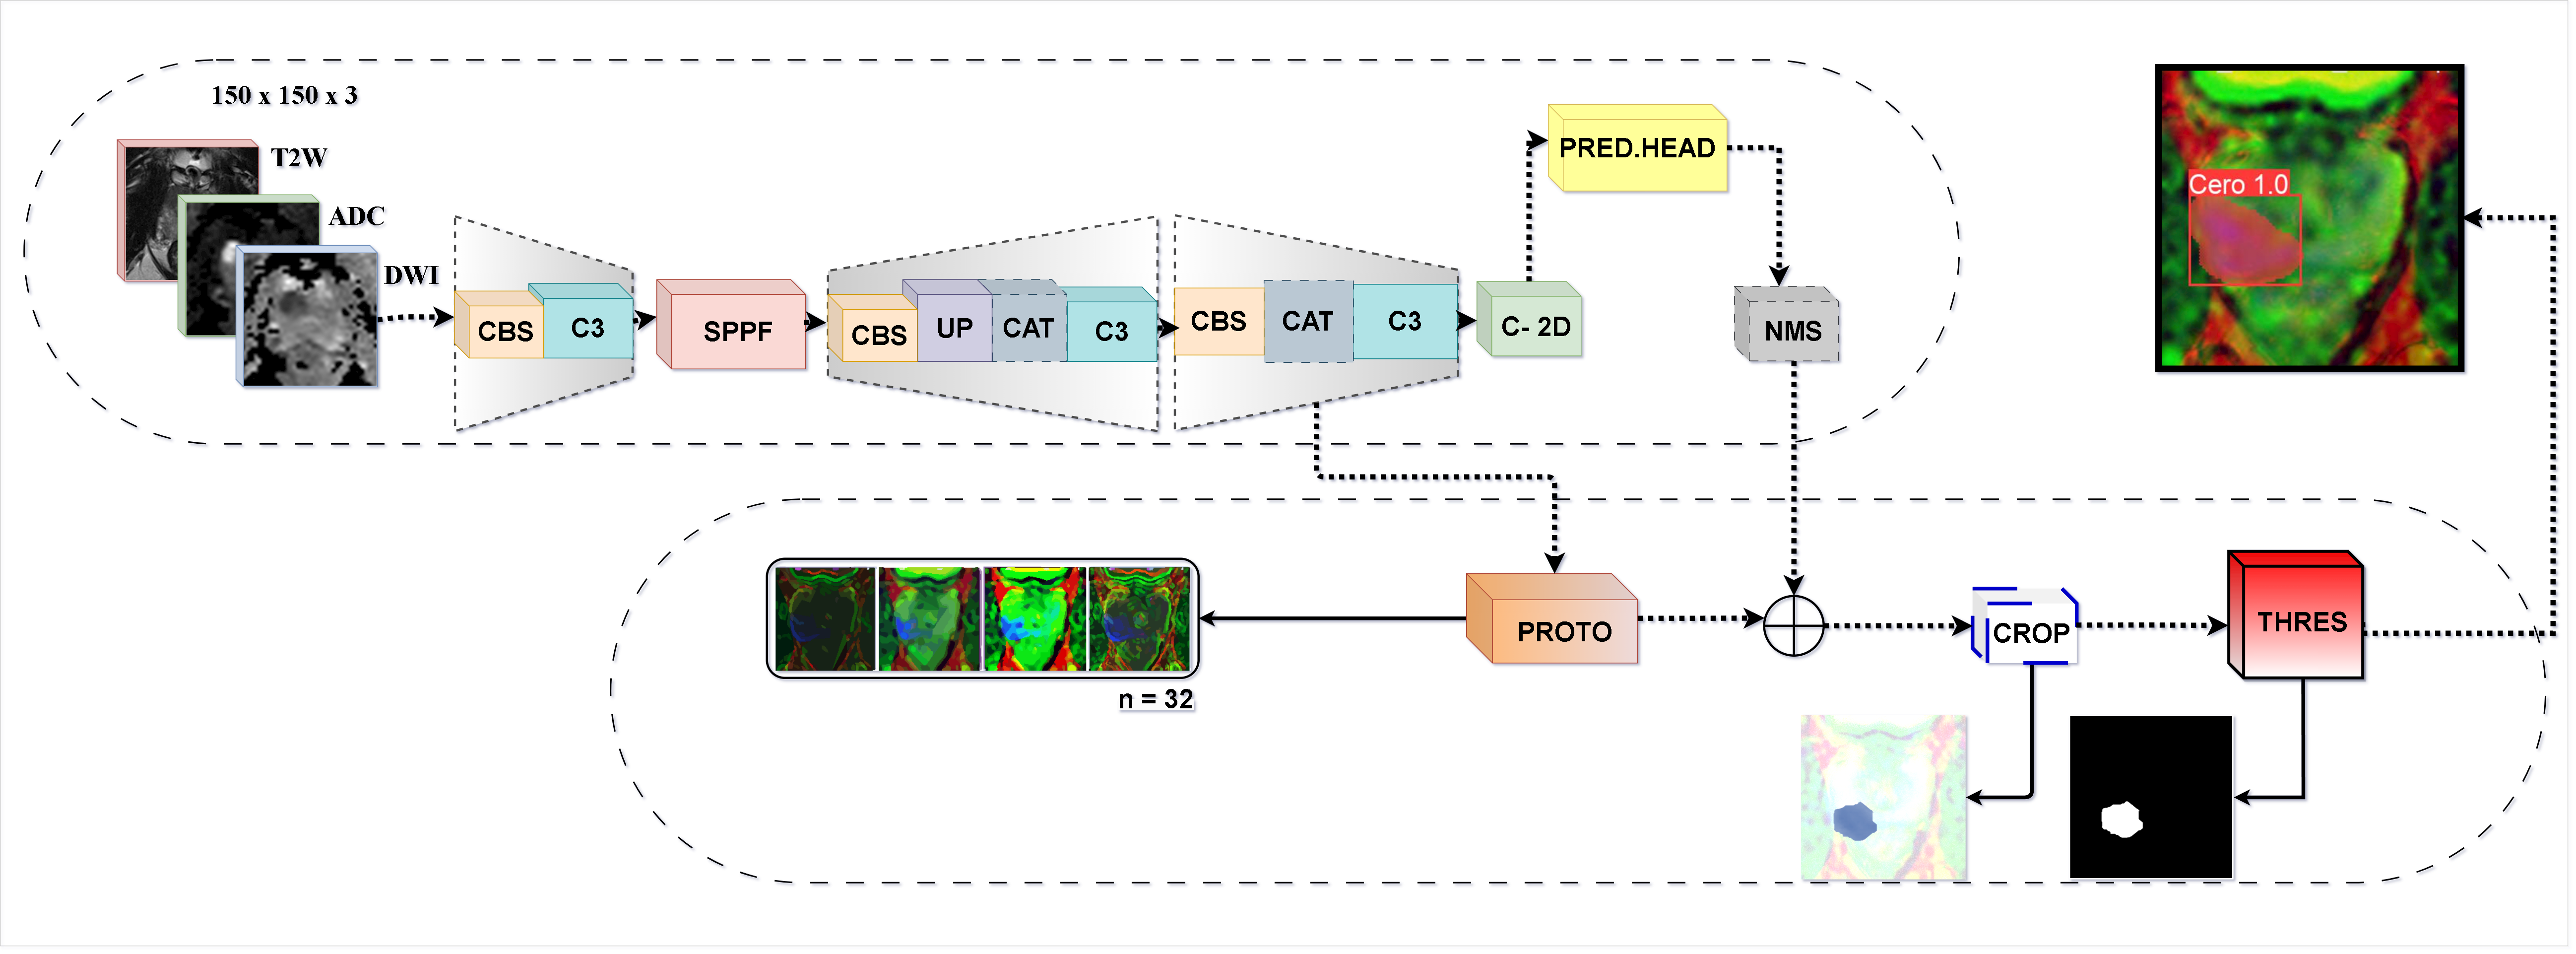
\includegraphics[width=1\textwidth]{imgs/pip_2.png}
	\label{fig:pipeline}
\end{figure}

\begin{figure}[h!]
	\noindent \textbf{Nota:} 
	% Figura construida con el uso de datos bp-MRI de próstata de centros médicos de los Países Bajos \footnote{PICAI_BIAS}, y  procesadas con el software ITK-SNAP \footnote{ITKSNAP}.
\end{figure}

% --> Figura del pipeline general [no es tan imporante ser muy detallado con cada componente... porque cada una de ella va a tener su propiea figura... pero si algo ilustrativo por ejempo pequeñas imagenes de activaciones...]

\section{Extracción de características}

% --> Estructura del backbone (incluyendo el upsample)... explicarlo [SPPSSS, y ettc los modulos que contenga..]

% ---> Figura para este bacbone

% ---> Figura con los mapas de saliencia 


\section{Predicción de regiones}

% --> Max supression...

% --> la cabaeza de prediccion [se entender cómo se llegó a los bounding...]

% ---> Figura para esta cabeza de prediccion

% --> La loss ...


\section{Contorno de lesiones para la tarea de localización}

En el procesamiento de imágenes médicas, la identificación precisa de las regiones de interés (ROI) es un componente crítico para el rendimiento óptimo de los modelos de aprendizaje automático. Así pues, se implementó un enfoque alternativo para el tratamiento de las anotaciones de las regiones con lesiones csPCA. En lugar de expandir el cuadro que delimita la lesión del radiólogo un 30\% normalizado, este enfoque implica la identificación de los puntos del perímetro de la lesión csPCA marcada por el radiólogo. Estos puntos se dilatan morfológicamente 5 píxeles, asegurando así que toda la lesión esté incluida. Posteriormente, se normalizan en relación con el tamaño de la máscara de referencia. Este enfoque ofrece una representación detallada de la lesión, lo cual puede potenciar la capacidad del modelo para aprender características relevantes. En términos más detallados, los puntos del perímetro de la lesión se mapean en el formato [Presencia de lesión, coordenada\_X1, Coordenada\_Y1, …, coordenada\_Xn, Coordenada\_Yn]. Este formato de anotaciones proporciona una representación precisa de las áreas de interés csPCA, asegurando que se disponga de la información más relevante para su uso en modelos de localización.

%--> cómo comolas involucra en la red


% ---> Figura sobre como se involucro la segmentacion


%--> Cómo cambió la loss... [se debe entender cómo la red está usando] 
\chapter{DISEÑO EXPERIMENTAL} %detalles de como usted armó su experimento

% --> del conjunta datos tomamos los que XXX condicion...

% --> redimensionados a XX tamano para introducirlos en la red...

% train val test split, cuantos casos o imagenes dejo en cada split [se fue precavido dejando del mismo en el mismo split]...

% learning... hyperparametros... numero de boxes... augmentation...

%----- si ud dice que hizo estas configuraciones: es porque usted luego en resultados va a mostrar o analizar esas configuraciones...


% se probó con diferentes secuencias ADC sola, DWI .. ADC+DWI, ...

% Se hizo con y sin segmentación...

% El tamaño de la glandula...

% \\begin{document}



% \begin{table}[h]
% \centering
% \captionsetup{justification=centering}
% \begin{tabular}{cccccc}
% \toprule
% \textbf{Secuencia} & \textbf{Precisión} & \textbf{Recall} & \textbf{Ap0.5} & \textbf{Ap .05-095} \\
% \midrule
% T2W & 0.452 & 0.258 & 0.255 & 0.0858 \\
% ADC & 0.68 & 0.516 & 0.538 & 0.197 \\
% DWI & 0.671 & 0.498 & 0.49 & 0.171 \\
% T2W-ADC-DWI & 0.746 & 0.535 & 0.588 & 0.228 \\
% \bottomrule
% \end{tabular}
% \caption{Comparativa de la utilización de diferentes secuencias, sin Fine Tunning}
% \label{tabla:ejemplo}
% \end{table}


% \begin{table}[h]
% \centering
% \captionsetup{justification=centering}
% \begin{tabular}{cccccc}
% \toprule
% \textbf{Secuencia} & \textbf{Precisión} & \textbf{Recall} & \textbf{Ap0.5} & \textbf{Ap .05-095} \\
% \midrule
% T2W & - & - & - & - \\
% ADC & 0.672 & 0.479 & 0.523 & 0.22 \\
% DWI & - & - & - & - \\
% T2W-ADC-DWI & - & - & - & - \\
% \bottomrule
% \end{tabular}
% \caption{Comparativa de la utilización de diferentes secuencias, Fine Tunning(Básico)}
% \label{tabla:ejemplo}
% \end{table}



% \begin{table}[h]
% \centering
% \captionsetup{justification=centering}
% \begin{tabular}{ccccccccccc}
% \toprule
% \textbf{Secuencia} & \multicolumn{4}{c}{\textbf{Sin Fine Tunning}} & \multicolumn{4}{c}{\textbf{Fine Tunning (Básico)}} & \multicolumn{2}{c}{\textbf{Cohorte de Prueba}} \\
%  & \textbf{Precisión} & \textbf{Recall} & \textbf{Ap0.5} & \textbf{Ap .05-095} & \textbf{Precisión} & \textbf{Recall} & \textbf{Ap0.5} & \textbf{Ap .05-095} & \textbf{Precisión} & \textbf{Recall} \\
% \midrule
% T2W & 0.452 & 0.258 & 0.255 & 0.0858 & - & - & - & - & - & - \\
% ADC & 0.68 & 0.516 & 0.538 & 0.197 & 0.672 & 0.479 & 0.523 & 0.22 & - & - \\
% DWI & 0.671 & 0.498 & 0.49 & 0.171 & - & - & - & - & - & - \\
% T2W-ADC-DWI & 0.746 & 0.535 & 0.588 & 0.228 & - & - & - & - & - & - \\
% \bottomrule
% \end{tabular}
% \caption{Comparativa de la utilización de diferentes secuencias}
% \label{tabla:ejemplo}
% \end{table}



% \begin{table}[h]
% \centering
% \captionsetup{justification=centering}
% \begin{tabular}{cccccc}
% \toprule
% \textbf{Secuencia} & \textbf{Precisión} & \textbf{Recall} & \textbf{Ap0.5} & \textbf{Ap .05-095} & \textbf{Tipo de Prueba} \\
% \midrule
% T2W & 0.452 & 0.258 & 0.255 & 0.0858 & Sin Fine Tunning \\
% ADC & 0.68 & 0.516 & 0.538 & 0.197 & Sin Fine Tunning \\
% DWI & 0.671 & 0.498 & 0.49 & 0.171 & Sin Fine Tunning \\
% T2W-ADC-DWI & 0.746 & 0.535 & 0.588 & 0.228 & Sin Fine Tunning \\
% T2W & - & - & - & - & Fine Tunning (Básico) \\
% ADC & 0.672 & 0.479 & 0.523 & 0.22 & Fine Tunning (Básico) \\
% DWI & - & - & - & - & Fine Tunning (Básico) \\
% T2W-ADC-DWI & - & - & - & - & Fine Tunning (Básico) \\
% T2W & - & - & - & - & Cohorte de Prueba \\
% ADC & - & - & - & - & Cohorte de Prueba \\
% DWI & - & - & - & - & Cohorte de Prueba \\
% T2W-ADC-DWI & - & - & - & - & Cohorte de Prueba \\
% \bottomrule
% \end{tabular}
% \caption{Comparativa de la utilización de diferentes secuencias}
% \label{tabla:ejemplo}
% \end{table}


% \begin{table}[h]
% \centering
% \captionsetup{justification=centering}
% \begin{tabular}{cccccc}
% \toprule
% \textbf{Secuencia} & \textbf{Precisión} & \textbf{Recall} & \textbf{Ap0.5} & \textbf{Ap .05-095} & \textbf{Tipo de Prueba} \\
% \midrule
% T2W & 0.452 & 0.258 & 0.255 & 0.0858 & Sin Fine Tunning \\
% ADC & 0.68 & 0.516 & 0.538 & 0.197 & Sin Fine Tunning \\
% DWI & 0.671 & 0.498 & 0.49 & 0.171 & Sin Fine Tunning \\
% T2W-ADC-DWI & 0.746 & 0.535 & 0.588 & 0.228 & Sin Fine Tunning \\
% T2W & 0.394 & 0.282 & 0.215 & 0.0543 & Sin Fine Tunning (Cohorte de Prueba) \\
% ADC & 0.745 & 0.436 & 0.479 & 0.184 & Sin Fine Tunning (Cohorte de Prueba) \\
% DWI & 0.669 & 0.342 & 0.429 & 0.163 & Sin Fine Tunning (Cohorte de Prueba) \\
% T2W-ADC-DWI & 0.74 & 0.496 & 0.566 & 0.251 & Sin Fine Tunning (Cohorte de Prueba) \\
% \midrule
% T2W & - & - & - & - & Fine Tunning (Básico) \\
% ADC & 0.672 & 0.479 & 0.523 & 0.22 & Fine Tunning (Básico) \\
% DWI & - & - & - & - & Fine Tunning (Básico) \\
% T2W-ADC-DWI & - & - & - & - & Fine Tunning (Básico) \\
% T2W & - & - & - & - & Fine Tunning (Básico, Cohorte de Prueba) \\
% ADC & - & - & - & - & Fine Tunning (Básico, Cohorte de Prueba) \\
% DWI & - & - & - & - & Fine Tunning (Básico, Cohorte de Prueba) \\
% T2W-ADC-DWI & - & - & - & - & Fine Tunning (Básico, Cohorte de Prueba) \\
% \bottomrule
% \end{tabular}
% \caption{Comparativa de la utilización de diferentes secuencias}
% \label{tabla:ejemplo}
% \end{table}



% \begin{table}[h]
% \centering
% \captionsetup{justification=centering}
% \begin{tabular}{cccccc}
% \toprule
% \textbf{Secuencia} & \textbf{Precisión} & \textbf{Recall} & \textbf{Ap0.5} & \textbf{Ap .05-095} & \textbf{Cohorte} \\
% \midrule
% T2W & 0.452 & 0.258 & 0.255 & 0.0858 & Validation \\
% ADC & {0.68} & {0.516} & {0.538} & {0.197} & Validation \\
% DWI & 0.671 & 0.498 & 0.49 & 0.171 & Validation \\
% T2W-ADC-DWI & {0.746} & {0.535} & \textbf{0.588} & \textbf{0.228} & Validation \\
% ADC-T2W-ADC & {0.445} & {0.433} & \textbf{0.46} & \textbf{0.24} & Validation \\
% ADC-DWI-ADC & {0.759} & {0.464} & \textbf{0.568} & \textbf{0.23} & Validation \\
% T2W-ADC-DWI-SEG+5 & {0.801}/0.814 & {0.563}/0.572 & \textbf{0.674}/0.696 & \textbf{0.333}/0.323 & Validation \\
% T2W-ADC-DWI-SEG & {0.797}/0.798 & {0.509}/0.509 & \textbf{0.594}/0.598 & \textbf{0.256}/0.244 & Validation \\
% \midrule
% T2W & 0.394 & 0.282 & 0.215 & 0.0543 & Test \\
% ADC & 0.745 & 0.436 & 0.479 & 0.184 & Test \\
% DWI & 0.669 & 0.342 & 0.429 & 0.163 & Test \\
% T2W-ADC-DWI & {0.74} & {0.496} & \textbf{0.566} & \textbf{0.251} & Test \\
% ADC-T2W-ADC & {0.707} & {0.368} & \textbf{0.504} & \textbf{0.24} & Test \\
% ADC-DWI-ADC & {0.75} & {0.393} & \textbf{0.553} & \textbf{0.247} & Test \\
% T2W-ADC-DWI-SEG+5 & {0.809}/0.809 & {0.539}/0.539 & \textbf{0.658}/0.655 & \textbf{0.348}/0.333 & Test \\
% T2W-ADC-DWI-SEG & {0.785}/0.799 & {0.458}/0.466 & \textbf{0.567}/0.575 & \textbf{0.29}/0.264 & Test \\

% \midrule
% T2W & - & - & - & - & Fine Tunning (Básico) \\
% ADC & \textbf{0.672} & \textbf{0.479} & \textbf{0.523} & \textbf{0.22} & Fine Tunning (Básico) \\
% DWI & - & - & - & - & Fine Tunning (Básico) \\
% T2W-ADC-DWI & - & - & - & - & Fine Tunning (Básico) \\
% T2W & - & - & - & - & Fine Tunning (Básico, Cohorte de Prueba) \\
% ADC & - & - & - & - & Fine Tunning (Básico, Cohorte de Prueba) \\
% DWI & - & - & - & - & Fine Tunning (Básico, Cohorte de Prueba) \\
% T2W-ADC-DWI & - & - & - & - & Fine Tunning (Básico, Cohorte de Prueba) \\


\begin{table}[h]
\centering
\captionsetup{justification=centering}
\begin{tabular}{cccccc}
\toprule
\textbf{Secuencia} & \textbf{Precisión} & \textbf{Recall} & \textbf{Ap0.5} & \textbf{Ap .05-095}  \\
\midrule
T2W & 0.394 & 0.282 & 0.215 & 0.0543 \\
ADC & 0.745 & 0.436 & 0.479 & 0.184 \\
DWI & 0.669 & 0.342 & 0.429 & 0.163 \\
T2W-ADC-DWI & {0.74} & {0.496} & \textbf{0.566} & \textbf{0.251} \\
T2W-ADC-DWI-(150\_150) & {0.514} & {0.479} & \textbf{0.56} & \textbf{0.251} \\
T2W-ADC-DWI-SEG-(150\_150) & {0.899} & {0.475} & \textbf{0.693} & \textbf{0.377} \\

% ADC-T2W-ADC & {0.707} & {0.368} & \textbf{0.504} & \textbf{0.24}  \\
% ADC-DWI-ADC & {0.75} & {0.393} & \textbf{0.553} & \textbf{0.247}  \\
% T2W-ADC-DWI-(150\_150) & {0.514} & {0.479} & \textbf{0.56} & \textbf{0.251} \\
% T2W-ADC-DWI-SEG+5 & {0.809}/0.809 & {0.539}/0.539 & \textbf{0.658}/0.655 & \textbf{0.348}/0.333 \\
% T2W-ADC-DWI-SEG & {0.785}/0.799 & {0.458}/0.466 & \textbf{0.567}/0.575 & \textbf{0.29}/0.264 \\
% T2W-ADC-DWI-SEG+5-(150\_150) & {0.899}/0.932 & {0.475}/0.492 & \textbf{0.693}/\textbf{0.705} & \textbf{0.377}/0.378 \\
% T2W-ADC-DWI-SEG+5-(150\_150\_NW) & {0.73}/0.772 & {0.527}/0.5 & \textbf{0.578}/0.566 & \textbf{0.279}/0.26 \\



\bottomrule
\end{tabular}
\caption{Comparativa de la utilización de diferentes secuencias}
\label{tabla:ejemplo}
\end{table}


\begin{table}[h]
\centering
\captionsetup{justification=centering}
\begin{tabular}{cccccc}
\toprule
\textbf{Threshold IOUV} & \textbf{Precisión} & \textbf{Recall} & \textbf{ApThreshold-0.95} & \textbf{ApThreshold-0.95}  \\
\midrule
0.1 & {0.673} & {0.627} & \textbf{0.727} & \textbf{0.523} \\
0.2 & {0.673} & {0.627} & \textbf{0.727} & \textbf{0.503} \\
0.3 & {0.902} & {0.5} & \textbf{0.722} & \textbf{0.468} \\
0.4 & {0.664} & {0.619} & \textbf{0.721} & \textbf{0.433} \\
0.5 & {0.899} & {0.475} & \textbf{0.693} & \textbf{0.377} \\
0.6 & {0.851} & {0.449} & \textbf{0.63} & \textbf{0.3} \\
0.7 & {0.692} & {0.364} & \textbf{0.497} & \textbf{0.204} \\
0.8 & {0.453} & {0.186} & \textbf{0.233} & \textbf{0.0969} \\
0.9 & {0} & {0} & \textbf{0} & \textbf{0} \\



\bottomrule
\end{tabular}
\caption{T2W-ADC-DWI-SEG-(150\_150) por Thresholds IOUv}
\label{tabla:ejemplo}
\end{table}


% \documentclass{article}
% \usepackage{tabularx}
% \usepackage{booktabs}
% \usepackage{caption}

% \begin{document}

% \begin{table}[h]
% \centering
% \captionsetup{justification=centering}
% \begin{tabularx}{\textwidth}{XXXXXX}
% \toprule
% \textbf{Secuencia} & \textbf{Precisión} & \textbf{Recall} & \textbf{Ap0.5} & \textbf{Ap .05-095} & \textbf{Tipo de Prueba} \\
% \midrule
% T2W & 0.452 & 0.258 & 0.255 & 0.0858 & Sin Fine Tunning \\
% ADC & \textbf{0.68} & \textbf{0.516} & \textbf{0.538} & \textbf{0.197} & Sin Fine Tunning \\
% DWI & 0.671 & 0.498 & 0.49 & 0.171 & Sin Fine Tunning \\
% T2W-ADC-DWI & \textbf{0.746} & \textbf{0.535} & \textbf{0.588} & \textbf{0.228} & Sin Fine Tunning \\
% ADC-T2W-ADC & \textbf{0.445} & \textbf{0.433} & \textbf{0.46} & \textbf{0.24} & Sin Fine Tunning \\
% \midrule
% T2W & 0.394 & 0.282 & 0.215 & 0.0543 & Sin Fine Tunning (Cohorte de Prueba) \\
% ADC & \textbf{0.745} & 0.436 & 0.479 & 0.184 & Sin Fine Tunning (Cohorte de Prueba) \\
% DWI & 0.669 & 0.342 & 0.429 & 0.163 & Sin Fine Tunning (Cohorte de Prueba) \\
% T2W-ADC-DWI & \textbf{0.74} & \textbf{0.496} & \textbf{0.566} & \textbf{0.251} & Sin Fine Tunning (Cohorte de Prueba) \\
% ADC-T2W-ADC & \textbf{0.707} & \textbf{0.368} & \textbf{0.504} & \textbf{0.24} & Sin Fine Tunning (Cohorte de Prueba) \\
% \bottomrule
% \end{tabularx}
% \caption{Comparativa de la utilización de diferentes secuencias}
% \label{tabla:ejemplo}
% \end{table}

% \end{document}



% \section{Conjunto de datos}

% Tres tipos de nanoespumas metálicas Cu-Ni fueron sintetizadas: $CuNi1$, $CuNi2$, $CuNi3$. Para esto se usaron tres diferentes soluciones acuosas con 1.5 M $H_{2}SO_{4}$ y diferentes concentraciones de $CuSO_{4} \cdot 5H_{2}O$ y  $NiSO_{4} \cdot 6H_{2}O$ para tener concentraciones de a) $0.3 M Cu^{2+}: 0.1 M Ni^{2+}$, b) $0.25 M Cu^{2+}: 0.15 M Ni^{2+}$ y c) $0.2 M Cu^{2+}: 0.2 M Ni^{2+}$. Estos tres tipos de nanoespumas fueron depositadas sobre un sustrato de cobre plano con un área de 1$cm^{2}$. Cada tipo de nanoespuma fue caracterizada usando un microscopio estereoscópico confocal con una magnificación de 700x. Finalmente, se capturaron un total de 600 imágenes de 1600 $\times$ 1200 pixeles constituyendo así un dataset balanceado con 200 imágenes por clase. Algunas muestras típicas de las imágenes microscópicas de nanoespumas capturadas se pueden ver en la figura \ref{fig:MNF_samples}.

% \begin{figure}[H]
%     \centering
%     \caption{Imágenes microscópicas de espumas metálicas nanoporosas Cobre-Níquel típicas.}
%     \label{fig:MNF_samples}
%      \begin{subfigure}[b]{0.3\textwidth}
%          \centering
%          \includegraphics[width=\textwidth]{imgs/Setup/cuni1_full.jpg}
%          \caption{Nanoespuma CuNi1}
%          \label{fig:CuNi_1_full}
%      \end{subfigure}
%      \hfill
%      \begin{subfigure}[b]{0.3\textwidth}
%          \centering
%          \includegraphics[width=\textwidth]
%          {imgs/Setup/cuni2_full.jpg}
%          \caption{Nanoespuma CuNi2}
%          \label{fig:CuNi_2_full}
%      \end{subfigure}
%      \hfill
%      \begin{subfigure}[b]{0.3\textwidth}
%          \centering
%          \includegraphics[width=\textwidth]
%          {imgs/Setup/cuni3_full.jpg}
%          \caption{Nanoespuma CuNi3}
%          \label{fig:CuNi_3_full}
%      \end{subfigure}        
% \end{figure}
\chapter{EVALUACIÓN Y RESULTADOS}

% Con respecto a los resultados con diferntes combinaciones... de secenacis MRI.. y con diferentes entradas de tmaanno de la glanduala... se entro que lo mejor es XX y XX ....

% A partir de esto nos quedamos CON xxx configuracion... y ahora con segmentación ... 







 



\chapter{CONCLUSIONES Y TRABAJO FUTURO}


% En este trabajo se implementó y adaptó un \textit{autoencoder} variacional para codificar patrones geométricos que correspondan a la síntesis de nanoespumas con diferentes composiciones. El autoencoder fue ajustado, siguiendo una tarea de reconstrucción de imágenes, y logrando codificar vectores embebidos con la capacidad de discriminación entre diferentes geometrías de las nanoespumas. 

% En este trabajo, utilizando observaciones de un microscopio confocal, se lograron observar patrones codificados en los vectores embebidos para representar patrones geométricos de las nanoespumas. Este hecho constituye un potencial de las herramientas computacionales para la caracterización y cuantificación de la geometría sin dedicarse a análisis tediosos y bajo medidas simplificadas de los poros.  Estos modelos son discriminables a partir del uso de herramientas de aprendizaje de máquina como \textit{Random Forest, KNN y decistion tree}, logrando niveles de precisión por encima del 90\%. 

% Además, los resultados evidencian que se pueden simular entornos experimentales para la construcción de nanoespumas, siendo este hecho de gran potencial en los expertos del área, para validar el comportamiento geométrico, frente a diferentes composiciones de cobre-níquel. Como herramienta alternativa, también se obtuvieron mapas de explicabilidad que pueden dar evidencia de los componentes geométricos que se codifican en el vector embebido. Así, logrando enfocarse en características como el espacio entre los poros y la geometría del poro, características usadas por los expertos durante el análisis. 

% Como trabajo futuro se esperan continuar indagando en nuevas arquitecturas que tengan la capacidad de representar la distribución de características geométricas, además que tengan el carácter discriminativo entre diferentes composiciones del material. También se pretende investigar el comportamiento con observaciones en otras magnificaciones, para que las herramientas computacionales puedan suplir requerimientos experimentales que pueden llegar a ser costosos o tomar tiempos prolongados en la síntesis de las nanoespumas.


% ------------------------------------------------------------------------
% Bibliografía
% ------------------------------------------------------------------------
\printbibliography[heading=bibintoc,title={BIBLIOGRAFÍA},omitnumbers=true] 
% ------------------------------------------------------------------------
% Anexos
% ------------------------------------------------------------------------
% ------------------------------------------------------------------------
% ------------------------------------------------------------------------
% ------------------------------------------------------------------------
%                                Anexo A
% ------------------------------------------------------------------------
% ------------------------------------------------------------------------
% ------------------------------------------------------------------------
% ------------------------------------------------------------------------
%\nnchapter{APPENDICES}
 % Artículos

% ------------------------------------------------------------------------
\end{document}                                          % Fin de documento
% ------------------------------------------------------------------------ 